%
% This is an example file and is hereby explicitly put in the
% public domain.
%
\documentclass[ppgc,diss,english]{iiufrgs}
% Para usar o modelo, deve-se informar o programa e o tipo de documento.
% Programas :
%   * cic       -- Graduação em Ciência da Computação
%   * ecp       -- Graduação em Ciência da Computação
%   * ppgc      -- Programa de Pós Graduação em Computação
%   * pgmigro   -- Programa de Pós Graduação em Microeletrônica
%
% Tipos de Documento:
%   * tc                -- Trabalhos de Conclusão (apenas cic e ecp)
%   * diss ou mestrado  -- Dissertações de Mestrado (ppgc e pgmicro)
%   * tese ou doutorado -- Teses de Doutorado (ppgc e pgmicro)
%   * ti                -- Trabalho Individual (ppgc e pgmicro)
%
% Outras Opções:
%   * english    -- para textos em inglês
%   * openright  -- Força início de capítulos em páginas ímpares (padrão da
%                   biblioteca)
%   * oneside    -- Desliga frente-e-verso
%   * nominatalocal -- Lê os dados da nominata do arquivo nominatalocal.def


% Use unicode
\usepackage[utf8]{inputenc}   % pacote para acentuação
%\usepackage[hyperpageref]{backref}

% Necessário para incluir figuras
\usepackage{graphicx}           % pacote para importar figuras
\usepackage{tikz}
\usetikzlibrary{positioning, calc, decorations.pathreplacing}
\usepackage{listofitems} % for \readlist to create arrays
\usetikzlibrary{arrows, arrows.meta} % for arrow size
\usepackage[outline]{contour} % glow around text
\contourlength{1.4pt}

\tikzset{>=latex} % for LaTeX arrow head
\colorlet{myred}{red!80!black}
\colorlet{myblue}{blue!80!black}
\colorlet{mygreen}{green!60!black}
\colorlet{myorange}{orange!70!red!60!black}
\colorlet{mydarkred}{red!30!black}
\colorlet{mydarkblue}{blue!40!black}
\colorlet{mydarkgreen}{green!30!black}
\tikzset{ % node styles, numbered for easy mapping with \nstyle
  my nodes/.style={circle,inner sep=0,minimum size=8mm},
  input/.style={my nodes,draw=mygreen,fill=mygreen!20,text=green!50!black},
  hidden/.style={my nodes,draw=violet,fill=violet!20,text=violet},
  output/.style={my nodes,draw=myred!60!black,fill=myred!20,text=red!60!black},
  my text/.style={text=#1,text width=1cm,align=center}
}

\usepackage{nicefrac}       % compact symbols for 1/2, etc.
\usepackage{amsfonts}       % blackboard math symbols
\usepackage{xspace}
\usepackage{amsmath}
\usepackage{amsthm}
\usepackage{amssymb}
\usepackage{algorithm}
\usepackage{algpseudocode}
\usepackage{varioref}
\usepackage[capitalise]{cleveref}
\usepackage{booktabs}       % professional-quality tables

% \usepackage{times}              % pacote para usar fonte Adobe Times
 \usepackage{palatino}
% \usepackage{mathptmx}          % p/ usar fonte Adobe Times nas fórmulas
%
\usepackage[alf,abnt-emphasize=bf]{abntex2cite} % pacote para usar citações abnt
\usepackage{subcaption}

\providecommand{\multiset}[1]{\ensuremath{\{\!\!\{#1\}\!\!\}}}
\providecommand{\sas}{\ensuremath{\text{SAS}^{+}}\xspace}
\providecommand{\strips}{STRIPS\xspace}
\providecommand{\astar}{\ensuremath{\text{A}^{*}}\xspace}
\providecommand{\gbfs}{\ensuremath{\text{GBFS}}\xspace}
\providecommand{\wida}{\ensuremath{\text{W-IDA}^{*}}\xspace}
\providecommand{\ida}{\ensuremath{\text{IDA}^{*}}\xspace}
\providecommand{\hvalue}[1]{\ensuremath{h^{#1}}\xspace}
\providecommand{\hstarp}[1]{\ensuremath{h^*({#1})}\xspace}
\providecommand{\hff}{\hvalue{\text{FF}}}
\providecommand{\hgc}{\hvalue{\text{GC}}}
\providecommand{\hstar}{\hvalue{*}}
\providecommand{\hlmc}{\hvalue{\text{lm-c}}}
\providecommand{\hmax}{\hvalue{\text{max}}}
\providecommand{\hadd}{\hvalue{\text{add}}}
\providecommand{\h}{$h$\xspace}
\providecommand{\hnn}{$\hat h$\xspace}
\providecommand{\hnrsl}{$\hat h^{\text{N-RSL}}$\xspace}
\providecommand{\hboot}{$\hat h^{\text{Boot}}$\xspace}
\providecommand{\hgc}{\hvalue{\text{gc}}}
\providecommand{\hhgn}{\hvalue{\text{HGN}}}
\providecommand{\unit}{/1\xspace}
\providecommand{\sui}{\text{SUI}\xspace}
\providecommand{\sai}{\text{SAI}\xspace}
\providecommand{\rw}{{RW}\xspace}
\providecommand{\bfs}{{BFS}\xspace}
\providecommand{\dfs}{{DFS}\xspace}
\providecommand{\bfsrw}{\text{FSM}\xspace}
\providecommand{\nn}{{NN}\xspace}
\providecommand{\fssp}{{FS}\xspace}
\providecommand{\bssp}{{BS}\xspace}
\providecommand{\hnnrs}{$\hat h{^{20\%}_\text{\meanfx}}$\xspace}
\providecommand{\hnnrsfifty}{$\hat h{^{50\%}_\text{\meanfx}}$\xspace}
\providecommand{\hffexp}{$h^{FF}_{exp}$}
\providecommand{\hgcexp}{$h^{GC}_{exp}$}
\providecommand{\hnnbase}{$\hat h_{0}$\xspace}
\providecommand{\hnnbfs}{$\hat h_{\text{bfs}}$\xspace}
\providecommand{\hnndfs}{$\hat h_{\text{dfs}}$\xspace}
\providecommand{\hnnrw}{$\hat h_{\text{rw}}$\xspace}
\providecommand{\hnnbfsrw}{$\hat h_\text{fsm}$\xspace}
\providecommand{\hnnbfsrwl}[1]{\ensuremath{\hat h_{#1}}\xspace}
\providecommand{\hnnnomutex}{\ensuremath{\hat h^{'}}\xspace}
\providecommand{\hnnnomutexl}[1]{\ensuremath{\hat h^{'}_{#1}}\xspace}
\providecommand{\hnnrsp}[1]{\ensuremath{\hat h_\text{fsm}/^{#1\%}_{\text{RS}}}\xspace}
\providecommand{\hnnrslp}[2]{\ensuremath{\hat h_\text{fsm}^{#1}/^{#2\%}_{\text{RS}}}\xspace}
\providecommand{\define}[1]{#1}
\providecommand{\facts}{\ensuremath{L_F}\xspace}
\providecommand{\meanfx}{\ensuremath{L_{\overline{F}}}\xspace}
\providecommand{\default}{\ensuremath{L_{200}}\xspace}
\providecommand{\distfarthest}{\ensuremath{d^*}\xspace}
\providecommand{\po}[1]{\ensuremath{\hat po^{#1}}\xspace}
\providecommand{\pot}[1]{\ensuremath{po^{#1}}\xspace}
\providecommand{\pog}{\po{\text{G}}}
\providecommand{\pofsm}{\po{\text{B}}}
\providecommand{\pogthresh}{\po{\text{G-thresh}}}
\providecommand{\pogmax}{\po{\text{G-max}}}
\providecommand{\popfa}{\po{\text{PFA}}}
\providecommand{\popfo}{\po{\text{PFO}}}
\providecommand{\postar}{\po{*}}
\providecommand{\postartable}{\pot{*}}
\providecommand{\pogstar}{\po{\text{G}^*}}
\providecommand{\pogstarthresh}{\po{\text{OPT-thresh}}}
\providecommand{\pogstarmax}{\po{\text{OPT-max}}}
\providecommand{\popf}{\po{\text{PF}}}
\providecommand{\poff}{\pot{\text{FF}}}
\providecommand{\pogc}{\po{\text{GC}}}

%% mathematical definitions
\ifcsname dom\endcsname\else\DeclareMathOperator{\dom}{Dom}\fi
\DeclareMathOperator{\pre}{pre}
\DeclareMathOperator{\eff}{eff}
\DeclareMathOperator{\sucs}{succ}
\DeclareMathOperator{\pred}{pred}
\DeclareMathOperator{\functioninitial}{initial\_state}
\DeclareMathOperator{\functiongoal}{goal\_condition}
\DeclareMathOperator{\mutex}{mutex}
\DeclareMathOperator{\del}{del}
\DeclareMathOperator{\add}{add}
\ifcsname R\endcsname\else\newcommand{\R}{\ensuremath{\mathbb{R}}}\fi


\providecommand{\floor}[1]{\ensuremath{\left\lfloor #1\right\rfloor}}
\providecommand{\ceil}[1]{\ensuremath{\left\lceil #1\right\rceil}}

\newtheorem{theorem}{Theorem}
\newtheorem{proposition}{Proposition}
\newtheorem{definition}{Definition}
\newtheorem{property}{Property}

% Hack to make todonotes use only the right margin
\makeatletter
\@mparswitchfalse%
\makeatother
\normalmarginpar

\usepackage[textsize=tiny,colorinlistoftodos,prependcaption,textwidth=width]{todonotes}

\newcommand{\mr}[2][noinline]{\todo[#1,fancyline,color=blue!20]{#2}}
\newcommand{\mri}[2][inline]{\todo[#1,fancyline,color=blue!20]{#2}}

\newcommand{\agp}[2][noinline]{\todo[color=orange!60,linecolor={orange!100},#1,fancyline,author=André]{#2}}
\newcommand{\agpi}[2][inline]{\todo[color=orange!60,linecolor={orange!100},#1,fancyline,author=André]{#2}}

\newcommand{\pp}[2][noinline]{\todo[color=purple!50,linecolor={purple!100},#1,fancyline,author=Pedro]{#2}}
\newcommand{\ppi}[2][inline]{\todo[color=purple!50,linecolor={purple!100},#1,fancyline,author=Pedro]{#2}}

% nominata
\renewcommand{\nominataReit}{Prof.~Carlos Andr{\'e} Bulh{\~o}es}
% \renewcommand{\nominataReitname}{Rector}
\renewcommand{\nominataPRCA}{Prof\textsuperscript{a}.~Patricia Pranke}
% \renewcommand{\nominataPRCAname}{Vice-Rector}
\renewcommand{\nominataPRAPG}{Prof.~J{\'u}lio Ot{\'a}vio Jardim Barcellos}
% \renewcommand{\nominataPRAPGname}{Dean of Graduate Studies}
\renewcommand{\nominataDir}{Prof\textsuperscript{a}.~Carla Maria Dal Sasso Freitas}
% \renewcommand{\nominataDirname}{Director of the Institute of Informatics}
\renewcommand{\nominataCoordPPGC}{Prof.~Alberto Egon Schaeffer Filho}
% \renewcommand{\nominataCoordnamePPGC}{Coordinator of the PPGC}
\renewcommand{\nominataBibchefe}{Alexsander Borges Ribeiro}
% \renewcommand{\nominataBibchefename}{Chief Librarian of the Institute of Informatics}


%
% Informações gerais
%
\title{Discovering and Learning Preferred Operators for Classical Planning with Neural Networks}
\translatedtitle{Descoberta e Aprendizado de Operadores Preferidos para Planejamento Clássico com Redes Neurais}

\author{Minini}{Pedro Probst}
% alguns documentos podem ter varios autores:
%\author{Flaumann}{Frida Gutenberg}
%\author{Flaumann}{Klaus Gutenberg}

% orientador e co-orientador são opcionais (não diga isso pra eles :))
\advisor[Prof.~Dr.]{Ritt}{Marcus}
\coadvisor[Prof.~Dr.]{Pereira}{André Grahl}

% a data deve ser a da defesa; se nao especificada, são gerados
% mes e ano correntes
%\date{maio}{2001}

% A seguir são apresentados comandos específicos para alguns
% tipos de documentos.

% Relatório de Pesquisa [rp]:
% \rp{123}             % numero do rp
% \financ{CNPq, CAPES} % orgaos financiadores

% Trabalho Individual [ti]:
% \ti{123}     % numero do TI
% \ti[II]{456} % no caso de ser o segundo TI

%
% palavras-chave
% iniciar todas com letras maiúsculas
%
\keyword{Classical planning}
\keyword{Heuristic search}
\keyword{Preferred operators}
\keyword{Machine learning}

%
% palavras-chave na lingua estrangeira
% iniciar todas com letras maiúsculas
%
\translatedkeyword{Planejamento clássico}
\translatedkeyword{Busca heurística}
\translatedkeyword{Operadores preferidos}
\translatedkeyword{Aprendizado de máquina}


%
% inicio do documento
%
\begin{document}

% folha de rosto
% às vezes é necessário redefinir algum comando logo antes de produzir
% a folha de rosto:
% \renewcommand{\coordname}{Coordenadora do Curso}
\maketitle

% dedicatoria
\clearpage
\begin{flushright}
\mbox{}\vfill
{\sffamily\itshape
    ``All this from a slice of gabagool?''\\}
--- \textsc{Tony Soprano}
\end{flushright}

% agradecimentos
\chapter*{Acknowledgements}

I would like to express my sincere gratitude to my advisors, Marcus Ritt and André G. Pereira, for their support and guidance throughout the duration of this two-year journey. I consider myself incredibly fortunate to have had such dedicated mentors.

I would also like to extend my appreciation to my colleague, Rafael V. Bettker, whose tireless dedication and ability to program long hours into the night have greatly contributed to the extensibility and success of our research.

Lastly, I want to express my deep gratitude to my mother for being the only family I have.

% abstract in english
\begin{abstract}
In a planning task, an agent must choose the most appropriate action from a potentially large set of actions at each step. Logic-based (or symbolic-based) planners use preferred operators to reduce the number of actions significantly. This work presents a method for sampling and learning preferred operators, ensuring their applicability across the entire state space of a planning task. We demonstrate that these learned preferred operators outperform the current best logic-based approach.
We aim to identify ideal preferred operators, which are situated along the shortest paths leading to some goal. However, due to the huge size of search state spaces, we introduce a novel sampling strategy tailored for extracting preferred operators. Our research shows that high-quality preferred operators can be obtained from a sample set covering only a fraction of the state space. Furthermore, a small neural network trained on these samples can effectively approximate ideal preferred operators.
To gain insights into this new category of preferred operators, we conduct controlled experiments: we systematically compare them to baselines, evaluate the effectiveness of preferred operators learned from several sample sizes, and assess their performance when combined with different heuristic functions.
\end{abstract}

% abstract in portuguese
\begin{translatedabstract}
Em uma tarefa de planejamento, um agente deve escolher a ação mais adequada de um conjunto potencialmente grande de ações em cada passo. Planejadores lógicos (ou simbólicos) usam operadores preferidos para reduzir significativamente o número de ações. Este trabalho apresenta um método para amostragem e aprendizagem de operadores preferidos, garantindo sua aplicabilidade em todo o espaço de estados de uma tarefa de planejamento. Demonstramos que esses operadores preferidos aprendidos superam a melhor abordagem lógicos atual.
Nosso objetivo é identificar os operadores preferidos ideais, que estão situados ao longo dos caminhos mais curtos que levam a algum objetivo. No entanto, devido ao enorme tamanho dos espaços de estado, apresentamos uma nova estratégia de amostragem adaptada para extrair operadores preferidos. Nossa pesquisa mostra que operadores preferidos de alta qualidade podem ser obtidos de um conjunto de amostras que abrange apenas uma fração do espaço de estados. Além disso, uma pequena rede neural treinada nessas amostras pode aproximar com eficácia os operadores preferidos ideais.
Para obter uma compreensão mais aprofundada sobre essa nova categoria de operadores preferidos, realizamos experimentos controlados: nós os comparamos sistematicamente com \textit{baselines}, avaliamos a eficácia dos operadores preferidos aprendidos com vários tamanhos de amostra e avaliamos seu desempenho quando combinados com diferentes funções heurísticas.
\end{translatedabstract}

% lista de abreviaturas e siglas
% o parametro deve ser a abreviatura mais longa
% A NBR 14724:2011 estipula que a ordem das abreviações
% na lista deve ser alfabética (como no exemplo abaixo).
\begin{listofabbrv}{SPMD}
        \item[BCE] Binary Cross-Entropy
        \item[BFS] Breadth-First Search
        \item[\bfsrs] Breadth Random Successors \pp{Needs a cooler/descriptive (but short) name. Accepting suggestions!}
        \item[BSS] Backward State Space
        \item[DFS] Depth-First Search
        \item[DTG] Domain Transition Graph
        \item[FSS] Forward State Space
        \item[FF] Fast-Forward
        %\item[FSM] Flying Spaghetti Monster
        \item[GBFS] Greedy Best-First Search
        \item[IPC] International Planning Competition
        \item[MSE] Mean Squared Error
        \item[MLP] Multi-Layer Perceptron
        \item[NN]  Neural Network
        \item[PDDL] Planning Domain Definition Language
        \item[ResNet] Residual Network
        \item[\sai] Sample Improvement
        \item[\sas] Simplified Action Structures Plus
        %\item[SD] Standard Deviation
        %\item[SPG] Shortest Path Graph
        \item[STRIPS] Stanford Research Institute Problem Solver
        \item[\sui] Successor Improvement
\end{listofabbrv}

\begin{listofsymbols}{$\alpha\beta\pi\omega$}
       %\item[$G$] Sample set graph
       %\item[$G'$] Shortest path sample set graph
       \item[$d^{*}$] Longest distance between the goal state and any potential initial state
       \item[\h] Heuristic
       \item[\hstar] Optimal heuristic
       \item[\hnn] Learned heuristic
       \item[\hadd] Add heuristic
       \item[\hff] FF heuristic
       \item[\hgc] Goal-count heuristic
       \item[\postartable] Oracle of ideal preferred operators
       \item[\postar] Learned ideal preferred operators
       \item[\poff] FF preferred operators
       \item[\pofsm] \bfsrw-based learned preferred operators
       \item[\pog] shortest-path-graph-based learned preferred operators
       \item[\pogstar] shortest-path-graph-based (with \hstar-values) learned preferred operators
\end{listofsymbols}

\listoffigures

\listoftables

\listofalgorithms

\tableofcontents

%
% - - - - - - - - - - - - - - - -- - - - - -
% intro
% - - - - - - - - - - - - - - - -- - - - - -
% introduce the problem,
% show why the problem is interesting,
% and how we attack it
%
\chapter{Introduction}
\label{cha:introduction}
In planning, preferred operators act in conjunction with heuristic functions and help reduce the number of expanded states during the planning process by prioritizing states closer to a goal condition.
This study introduces a novel approach to deriving preferred operators in planning tasks. Unlike the traditional logic-based methods, we use a sample-based approach to discover preferred operators. By training a neural network (NN) with a sample set consisting of pairs of states and their preferred operators discovered during the sampling procedure, the NN learns to generalize preferred operators for the given planning task.

\section{Planning}
\label{sec:intro-planning}
Planning involves determining a series of operators (or actions) that transitions a given initial state to a desired goal state.
In a classical planning task, the agent acts in a fully-observable environment, i.e., with access to all relevant information of the current state of the world, such as the positions of objects and the values of variables. The agent starts in a initial state and needs to fulfill a specific goal condition. This is achieved by using deterministic operators to modify the current state of the world. A solution plan for the planning task can be defined as a sequence of operators that, when applied to the initial state, successfully satisfy the goal condition. A state expansion involves the application of all relevant operators to a given state, thereby generating its successor states.

For example, in a Blocks World task, consider the initial state (left) and the goal state (right) shown in Figure \ref{fig:intro-blocks}. The agent needs to apply a sequence of operators to reach the goal state from the initial state. We can define operators such as ``pick up block X'', ``put block X on block Y'', and ``put block X on the table.'' In this example, the agent can find one of the possible plans by applying the following operators: pick up block G, put block G on the table, pick up block B, put block B on block G, and put block R on block B. %Applying each of these operators generate a successor state.

\begin{figure}[ht]
\caption[Initial state of a Blocks World task]{Initial state and goal state of a Blocks World task.}
\vspace{\baselineskip}
\centering
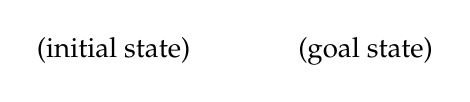
\begin{tikzpicture}
  % Initial state
  \node[align=center] at (7,-0.3) {(initial state)};
  \drawCube{7}{0.5}{0}{R}{red}{0.7}
  \drawCube{7}{1.2}{0}{B}{blue}{0.7}
  \drawCube{7}{1.9}{0}{G}{green}{0.7}

  % Goal state
  \node[align=center] at (10.2,-0.3) {(goal state)};
  \drawCube{10}{0.5}{0}{G}{green}{0.7}
  \drawCube{10}{1.2}{0}{B}{blue}{0.7}
  \drawCube{10}{1.9}{0}{R}{red}{0.7}
\end{tikzpicture}
\label{fig:intro-blocks}
\end{figure}

Planning tasks are solved by planners, which are software systems designed to find plans for given planning problems. Planners use several algorithms and techniques to explore the search space of possible operators and states in order to find an optimal or satisfactory plan. Planners typically take as input a formal representation of the planning problem, including the initial state, goal condition, and a set of available operators. The formal representation of a planning task can be specified using various notations~(\cref{sec:background-planning-notation}).

\section{Heuristic Search}
\label{sec:intro-heuristic-search}
%To solve planning tasks, planners commonly use a best-first search algorithm, which uses a function~$f$ to guide the search. The function $f$ combines the current cost $g(s)$ of a partial sequence of operations initiated from the initial state and reaching state $s$, along with a heuristic function $h(s)$~(\cref{sec:background-heuristics}) that provides an estimate of the cost-to-goal (also known as heuristic value or $h$-value) from state $s$.

Most planners are based on a best-first search algorithm such as greedy best-first search (GBFS)~\cite{Doran.Michie/1966}. GBFS arranges states in a priority queue based on their cost-to-goal estimate (also known as heuristic value or $h$-value) provided by the heuristic function. It explores states with the lowest cost-to-goal estimate first in order to find a solution. Various domain-independent heuristics effectively calculate the cost-to-goal estimate of a state by using domain logic, which has information that permits reasoning about operators and other rules, such as mutexes that indicate infeasible states. These heuristics are based mainly on techniques such as abstractions~\cite{Culberson.Schaeffer/1998}, delete relaxation~\cite{Hoffmann.Nebel/2001}, and landmarks~\cite{Hoffmann.etal/2004,Helmert.Domshlak/2009}. The heuristic function is the most important component of a planner since it guides the search.

\section{Preferred Operators}
\label{sec:intro-preferred-ops}
Operators that are deemed favorable for specific reasons, such as generating states that are closer to the goal, are referred to as preferred operators~\cite{Helmert/2006,Richter.Helmert/2009}. These operators are used alongside heuristic functions to assist planners in minimizing the number of expanded states when solving a planning task.
By prioritizing the expansion of states generated by preferred operators, planners benefit from additional guidance, often resulting in a higher success rate for solving tasks compared to only relying on the heuristic function. Learning preferred operators shares similarities with learning policies, as both involve the selection of actions that are more likely to result in desirable outcomes. The existing methods for identifying preferred operators are currently limited to logic-based approaches. The most effective approach used at present involves using the preferred operators calculated alongside the Fast-Forward (FF) heuristic~\cite{Hoffmann.Nebel/2001}, as implemented in the Fast Downward planning system~\cite{Helmert/2006}. Planners incorporating preferred operators emerged as winners in the satisficing track of the International Planning Competition (IPC) in 2004, 2008, 2011, and 2018~\cite{Helmert/2006,Richter.lama.etal/2011,Richter.lama.etal/2011,Seipp-fast.etal/2018}.

\section{Deep Learning}
\label{sec:intro-deep-learning}
Deep learning is a subfield of machine learning that focuses on the design and training of NNs with multiple layers~\cite{Goodfellow.etal/2016}. It revolves around the concept of learning hierarchical representations of data, where each layer in the network progressively extracts more complex and abstract features. Through the use of NNs, learning algorithms can automatically discover and capture patterns from large-scale datasets in a variety of tasks, including image classification, speech recognition, and natural language processing.

Deep learning models can learn in different ways. This study focuses on supervised learning, which involves using labeled datasets to classify or make predictions. In this case, a dataset used to train an NN can be represented as multiple pairs in the format $(y, x)$. Here, the target $y$ refers to the desired output or label associated with a specific input instance $x$. Learning models can effectively learn and generalize from the provided labeled data to make accurate predictions or classify new, unseen inputs.

\section{Learning in Planning}
\label{sec:intro-learning-planning}
In recent years, interest in using NNs to learn heuristic functions~\cite{Ferber.etal/2020a,Yu.etal/2020,Shen.etal/2020,Ferber.etal/2022,OToole/2022} or policies~\cite{Toyer.etal/2018,Toyer.etal/2020,Stahlberg.etal/2022} to solve planning tasks has increased. For supervised methods, the general approach is to generate a set of samples as pairs of states and cost-to-goal values and use them to train an NN. However, it is challenging to learn effective heuristic functions, since state spaces tend to grow exponentially in size as the amount of information needed to describe them increases, but the portion of the state space that we can actually sample is relatively small. Also, logic-based heuristics can be applied to any domain, while learned heuristics depend on the learning model, and even with domain-independent models, transfer learning can be difficult~\cite{Shen.etal/2020}. Moreover, learned heuristics are generally slow to compute, thus they need to be more informed, i.e., expand fewer states when compared to logic-based heuristics to reach the goal. These challenges also apply to learning preferred operators.

\section{Contributions}
\label{sec:intro-contributions}
This study represents the first attempt to discover preferred operators from a sample set and use an NN to learn them. We present a new sampling method and a novel sample-based technique for identifying preferred operators. The technique involves backward search from the goal (also known as regression), constructing a graph with sampled states representing their successor-predecessor relationships, and determining for each state the set of operators used to reach the goal as preferred operators. We show that an NN can learn the preferred operators from a subset of the state space and effectively extend this learning to the entire state space across diverse planning domains. Furthermore, the proposed approach outperforms the current best logic-based preferred operator method in the benchmark tasks. In particular, this work presents:

\begin{itemize}
\item A novel method based on shortest path graphs to discover preferred operators in an existing sample set~(\cref{sec:sample-discovered-po}).
\item A new sampling method tailored for discovering preferred operators~(\cref{sec:sample-learn-po}).
\item An analysis of the quality of the learned preferred operators and a comparison to existing logic-based methods~(\cref{cha:exp-experiments}).
\end{itemize}
%
% - - - - - - - - - - - - - - - -- - - - - -
% background
% - - - - - - - - - - - - - - - -- - - - - -
% these are all things that exist already
% and that the reader needs to know before
%
\chapter{Background}
\label{cha:background}
This chapter provides essential information for comprehending the subsequent chapters of this work.

\section{Classical Planning Notation}
\label{sec:background-planning-notation}
In this section we present three ways to represent a classical planning task. The first one, STRIPS~\cite{Fikes.Nilsson/1971}, represents a planning task using propositional facts (Boolean variables). The second way, \sas~\cite{Backstrom.Nebel/1995}, represents a planning task using multi-valued state variables. The third way, PDDL~\cite{Ghallab.etal/1998}, is based on predicate logic and is commonly used for writing planning tasks to be used as input for planners.

\subsection{STRIPS}
\label{sec:background-strips}
% A planning task in STRIPS is defined as $\Pi = \langle F, O, I, G\rangle$ where $F$ is a set of facts (Boolean variables), $O$ is a set of operators or actions over $F$, where $\langle Pre(o), Add(o), Del(o) \rangle \subseteq F$, $I \subseteq F$ is the initial state, and $G \subseteq F$ is a a set of goal facts that must be satisfied. We say that operators $O(s)$ are \emph{applicable} in $s$ if they satisfy $Pre(o)$. We progress a state $s$ with operator $o$ by setting the propositions in $Add(o)$ to true and $Del(o)$ to false. Finally, a sequence of operators $\pi=(o_1,\ldots,o_k)$ applicable to the initial state is called a plan.
\begin{definition}[STRIPS Planning Task]\label{def:strips}
A planning task in STRIPS representation is defined by~$\Pi=\langle\mathcal{P},\mathcal{O},s_{0},s^{*}\rangle$, where $\mathcal{P}$~is a set of propositions, $\mathcal{O}$~is a set of operators,~$s_{0} \subseteq \mathcal{P}$ is an initial state, and~$s^{*}$ is the goal condition.
A state $s$ is defined as $s \subseteq \mathcal{P}$, where each proposition in $s$ can be true ($p \in s$) or false ($p \notin s$). %The set~$\mathcal{S}$ of all states over $\mathcal{P}$ is the state space.
An operator~$o \in \mathcal{O}$ is defined by a triple~$\langle\pre(o),\add(o),\del(o)\rangle$ that specifies its preconditions, add-effects and delete-effects, respectively.
\end{definition}

In STRIPS, we say that operator $o$ is applicable to state $s$ if its preconditions are satisfied by $s$, i.e., $\pre(o) \subseteq s$, and produces a successor state~$s' = \sucs(s,o) = (s \setminus \del(o)) \cup \eff(o)$. In other words, we progress a state $s$ with operator $o$ by setting the propositions in $\del(o)$ to false and in $\add(o)$ to true. The set of successor states of $s$ is denoted by~$\sucs(s)=\{\sucs(s,o)\mid o\in \mathcal{O}, \pre(o) \subseteq s\}$.

\begin{definition}[Plan]\label{def:plan}
A sequence of operators~$\pi=(o_1,\ldots,o_k)$ is valid for a state~$s_0$ if produces a sequence of states~$s_1,\ldots,s_k$ such that $s_i=\sucs(s_{i-1},o_i)$. A sequence~$\pi$ for the initial state~$s_{0}$ is called a plan if $s^{*} \subseteq s_{k}$. The plan length is defined as $|\pi|$. Among all the valid plans, the one with the minimum length is referred to as an optimal plan. An optimal plan is the shortest plan that successfully achieves the goal state from the initial state.
\end{definition}

Heuristics based on delete-relaxation obtain the heuristic from a \emph{relaxed} version of the planning task. A relaxed planning task in STRIPS is defined as $\Pi^{+}=\langle\mathcal{P},\mathcal{O'},s_{0},s^{*}\rangle$, where $\mathcal{O'} = \{ \langle \pre(o), \add(o), \emptyset \rangle \,|\, o \in O \}$, i.e., the delete-effects of the planning task are ignored. Relaxed tasks can be solved efficiently even though finding the optimal solution is $\mathcal{NP}$-hard~\cite{Bylander/1994}. For example, the heuristic \hadd approximates the optimal heuristic value for a state $s$ as the sum of the costs of achieving each proposition in $s^{*}$ independently of the others.

\subsection{\sas}
\label{sec:background-sas}
We also use the \sas representation to describe classical planning tasks independent of any particular domain.

\begin{definition}[\sas Planning Task]\label{def:sas}
A \sas task is defined as $\Pi=\langle\mathcal{V},\mathcal{O},s_0,s^*\rangle$, where $\mathcal{V}$ is a set of state variables, and each variable $v\in \mathcal{V}$ has a finite domain~$\dom(v)$, that represents a set of mutually exclusive propositions called mutexes (variables from different domains can also be mutexes), $\mathcal{O}$ is a set of operators where each operator $o \in \mathcal{O}$ is defined as a pair of preconditions and effects $(\pre(o),\eff(o))$, both partial states~$s$ defined as a partial function $s:\mathcal{V}\rightarrow \mathcal{D}$, where $\mathcal{D}=\cup_{v\in \mathcal{V}}\dom(v)$, such that $s(v)\in \dom(v)$ whenever $s(v)$ is defined. Otherwise, $s(v)$ is undefined and written as $s(v)=\bot$.  A (complete) state $s$ is a partial state defined on all variables in~$\mathcal{V}$. The state~$s_0$ defines the initial state, and the partial state~$s^*$ defines the goal condition. %where $s_0, s^* \in \mathcal{S}$ and $\mathcal{S}$ is the set of all states (or state space).
%the expression $\mathcal{D}=\cup_{v\in \mathcal{V}}\dom(v)$ means that the domain of $\mathcal{D}$ is the union of the domains of all the elements in $\mathcal{V}$. That is, the set of values that $\mathcal{D}$ can take is the combination of all the values that each element in $\mathcal{V}$ can take.
\end{definition}

An operator $o \in \mathcal{O}$ is applicable to a state $s$ if its preconditions are fulfilled by $s$, denoted by $\pre(o) \subseteq s$, and it generates a successor state $s'=\sucs(s,o):=\eff(o)\circ s$. Here, $s'=t\circ s$ is defined as $s'(v)=t(v)$ for all $v$ such that $t(v)$ is defined, and for all other cases, $s'(v)=s(v)$. The set of all successor states resulting from state $s$ is denoted by $\sucs(s)=\{{\sucs(s,o)\mid o\in \mathcal{O}, \pre(o) \subseteq s}\}$.%A sequence of operators $\pi=(o_1,\ldots,o_k)$, where $o_i\in \mathcal{O}$, is considered valid for the initial state $s_0$ if, for $i\in[k]$, operator $o_i$ can be applied to $s_{i-1}$, and produces $s_i=\sucs(s_{i-1},o_i)$. %A plan refers to a valid sequence $\pi$ for $s_0$ such that $s^* \subseteq s_k$. In this work, all operators have unit costs, so the plan length is $|\pi| = k$.

\subsection{PDDL}
\label{sec:background-pddl}
We can also represent a classical planning task using PDDL. Tasks specified in PDDL are written in a Lisp-like syntax and are separated into two definitions, the domain, which specifies the operators and predicates, and the task, which specifies the objects, the initial state, and the goal condition.

\begin{definition}[PDDL Domain]\label{def:pddl-domain}
A PDDL domain is defined as a tuple $D = (\mathcal{P}, \mathcal{O})$, where $\mathcal{P}$ is a set of predicates representing the state of the world. Each predicate $p \in \mathcal{P}$ can be true or false in a given state. The set of operators is defined as $\mathcal{O}$. Each operator $o \in \mathcal{O}$ has a pre-condition $\pre(o)$ and an effect $\eff(o)$.
\end{definition}

In PDDL, effects are not explicitly separated into add-effects and delete-effects, instead, delete-effects are represented by negating the predicates.

\begin{definition}[PDDL Task]\label{def:pddl-domain}
A PDDL task is a triple $T = (D, s_{0}, s^{*})$, where $D$ is the domain definition associated with the problem, $s_{0}$ is the initial state, represented as $s_{0} = \{p_1, p_2, \ldots, p_n\}$, where $p_i \in \mathcal{P}$, and $s^{*}$ is the goal condition, denoted as $s^{*} = \{q_1, q_2, \ldots, q_m\}$, where $q_i \in \mathcal{P}$ represents the desired state of predicate $q_i$ to be achieved.
\end{definition}

%Actions represent the possible operations or transformations that can be performed, while predicates describe the properties or conditions that can be true or false within the domain. Objects are the entities involved in the planning task, while the initial state describes the starting configuration or state of the objects. The goal condition defines the desired state that a planner aims to achieve.

As an example, consider Blocks World, where $(ontable~?x)$ represents a predicate that indicates if a block $x$ is on the table or not, and $(pickup~?x)$ is an action that defines the act of picking up block $x$. This action is further specified by a set of preconditions $(and~(clear~?x)~(ontable~?x)~(handempty))$ that must hold true before $(pickup~?x)$ is applied, i.e., $x$ must be clear (no other block above it), $x$ must be on the table, and the hand must be empty. The effects of applying $(pickup~?x)$ are $$(and~(not~(ontable~?x))~(not~(clear~?x))~(not~(handempty))~(holding~?x)),$$

that is, $x$ is not on the table, $x$ is not clear, the hand is not empty, and the hand is holding $x$.

\section{Regression}
\label{background-regression}

The predecessor of a partial state $s$ under operator $o$, denoted $\pred(s,o)$, can be obtained through a process called backward search or regression. Regression involves determining predecessor states that can lead to the current partial state by applying the operator $o$. An operator $o$ is considered relevant for partial state $s$ if at least one defined effect in $o$ is applicable to $s$, i.e., there exists at least one effect in the operator $o$ whose preconditions are satisfied by the partial state $s$, and consistent if the operator agrees with the defined effects in $s$. An operator $o$ is said to be \emph{backward applicable} in partial state $s$ if it is both relevant and consistent with $s$, and it leads to a predecessor $r$ given by $r=\pre(o)\circ (s|_{\dom(s)\setminus\eff_r})$\pp{$eff_r$ or $eff_o$?}. Note that $\sucs(r,o)\subseteq s$ may differ from $s$, i.e., applying an operator to a predecessor state may result in a subset of the current partial state, but it does not necessarily cover all the possible states represented by $s$.
% $(s|_{\dom(s)\setminus\eff_r})$: This part refers to the restriction or projection of the current partial state $s$ onto the variables in its domain ($\dom(s)$) that are not affected by the effects of operator $o$ ($\eff_r$). In other words, it selects the values of the variables in $s$ that are not modified by $o$.
A partial state $s$ has predecessors $\pred(s)=\{{\pred(s,o)\mid o\in \mathcal{O}}\}$ where $o$ is backward applicable to $s$, and a regression sequence from state $s_0$ is valid if $o_i$ can be applied to $s_{i-1}$ and produces $s_i=\pred(s_{i-1},o_i)$. All partial states~$s_k$ can reach a partial state $s\subseteq s_0$ in at most $k$ forward applications of the reversed operator sequence.
If a valid regression sequence $\rho = (o_1, \ldots, o_k)$ is generated, it will produce a sequence of partial states that can reach the goal state $s^*$ within a maximum of $k$ steps.



\section{State Spaces}
\label{background-state-spaces}

Let $S$ be a set of states, $s_0 \in S$ be an initial state, $s^{*} \in S$ be a goal state, and $\sucs : S \to 2^S$ be a successor function, which maps each state to a set of possible successor states and determines the available transitions. A state space is a tuple $X = \langle S, s_0, s^{*}, \sucs \rangle$.
\begin{definition}[State Space of $\Pi$]
For any planning task $\Pi$ with states $S$, initial state $s_0$, goal state $s^{*}$, and successor function $\sucs$, the corresponding state space of $\Pi$ is denoted as $X(\Pi) = \langle S, s_0, s^{*}, \sucs \rangle$.
\end{definition}

The forward state space (FSS) refers to the set of states that can be reached from the initial state $s_0$ by applying the successor function $\sucs$ in the forward direction. It represents the states that can be explored forward from the initial state towards the goal state.

\begin{definition}[Forward State Space of $\Pi$]
The forward state space for a planning task $\Pi$ is denoted as $X_{\text{F}}(\Pi) = \langle S_{\text{F}}, s_0, s^{*}, \sucs \rangle$, where $S_{\text{F}}$ is the set of states reachable from the initial state, and $\sucs : S_{\text{F}} \to 2^{S_{\text{F}}}$ is the successor function that maps each state to a set of possible successor states and determines the available transitions in the forward direction.
\end{definition}

In other words, $X_{\text{F}}(\Pi)$ is defined as the subset of states and transitions within $X$ that are relevant to the planning task $\Pi$ and the forward exploration towards the goal state. The FSS is explored when solving a task, for example by using a best-first search algorithm.

The backward state space (BSS), on the other hand, refers to the set of states that can be reached from the goal state $s^{*}$ by applying a predecessor function $\pred$. It represents the states that can be explored backward from the goal state towards the initial state~(\cref{background-regression}).

\begin{definition}[Backward State Space of $\Pi$]
 The backward state space of a planning task $\Pi$ is denoted as $X_{\text{B}}(\Pi) = \langle S_{\text{B}}, s_{0}, s^{*}, \pred \rangle$, where $S_{\text{B}}$ is the set of states reachable from the goal state and $\pred : S_{\text{B}} \to 2^{S_{\text{B}}}$ is a predecessor function that maps each state to a set of possible predecessor states and determines the available transitions in the backward direction.
\end{definition}


\section{Heuristic Functions}
\label{sec:background-heuristics}
A heuristic function $h:\mathcal{S}\rightarrow \mathbb{R}^{\geq 0}\cup\{\infty\}$ estimates the optimal plan length from a state $s$ to the goal $s^*$, where the optimal heuristic function is defined as $\hstar(s) = |\pi_{s}^{*}|$, i.e., the length of the true plan from $s$ to $s^{*}$. Heuristic functions are used to guide search algorithms, optimization techniques, or decision-making processes by providing informed estimates or approximations based on available information or problem-specific knowledge. The goal of a heuristic function is to efficiently guide the search or decision-making process towards more promising paths or solutions, even in the absence of complete or perfect information. A heuristic function can have several properties that indicate its quality, such as:

\begin{itemize}
        \item Admissibility: $h(s) \le \hstar{(s)}$, i.e., the heuristic never overestimates the true cost-to-goal.
        \item Consistency (or monotonicity): $h(s) \le h(s') + cost(o)$ for all transitions from a state $s$ to a successor $s'$, i.e., $s \xrightarrow{o} s'$, where $cost(o)$ is the cost of applying operator $o$ to reach $s'$ from $s$.
        \item Goal-awareness: $h(s) = 0$ for all goal states.
        \item Safeness: all states have $h(s) = \infty$ if $\hstar (s) = \infty$, for example in dead-ends.
\end{itemize}

Heuristics are typically derived from a model of the task, such as the \sas model introduced earlier, but can also be obtained by learning the map of some state $s$ to its heuristic value $h(s)$, where the desired output of the NN can be either the direct cost-to-goal estimates or some form of encoding representing these estimates.
\ppi{The paragraph below needs to change a bit since it's too similar to Rafael's.}
A propositional representation of a state is better suited for learning heuristic functions over states. For this purpose, consider a planning task denoted as $\Pi=\langle\mathcal{V},\mathcal{O},s_0,s^*\rangle$. Here, $\mathcal{V}=\{v_1,\ldots,v_n\}$ represents a set of variables, and $D(v_i)=\{d_{i1},\ldots,d_{i,s_i}\}$ represents the domains of variable $v_i$, with $i\in[n]$. To represent any state $s$, we use a sequence of facts denoted as
% The domain consists of possible values that $v_i$ can take. The values are represented as $d_{i1}$ to $d_{i,s_i}$, where $s_i$ indicates the number of possible values for $v_i$.
$$\mathcal{F}(s)=(f_{11},f_{12},\ldots,f_{1,s_1},\ldots,f_{n1},f_{n2},\ldots,f_{n,s_n}),$$ where each fact $f_{ij}=[s(v_i)=d_{ij}]$ indicates whether variable $v_i$ assumes the value $d_{ij}$ in state $s$. It is important to note that the facts $\mathcal{F}_i=\{f_{i1},\ldots,f_{i,s_i}\}$ corresponding to variable $v_i$ adhere to the consistency condition $\sum_{f\in \mathcal{F}_i} f\leq 1$, as each variable can take at most one value, and $\sum_{f\in \mathcal{F}_i} f=0$ only when $v_i$ is undefined.

For example, let $\mathcal{P}$ be a set of propositions, and let $p_i, p_j \in \mathcal{P}$ be two propositions. We say that $p_i$ and $p_j$ are mutex (mutually exclusive) if $\neg(p_i \land p_j)$ holds, i.e., $p_i$ and $p_j$ cannot both be true at the same time in any valid state of the planning problem. More generally, we express $\mutex(\mathcal{P})$ when the constraint $\sum_{p\in \mathcal{P}} [p]\leq 1$ must be satisfied within the states of $\Pi$. Planning systems can typically deduce mutexes from the description of the planning task $\Pi$~\cite{Helmert/2009}.


\section{Greedy Best-First Search}
\label{sec:background-gbfs}
Greedy Best-First Search (GBFS, \cref{alg:gbfs}) is a best-first search algorithm typically used by planners to solve planning tasks by exploring the FSS. GBFS organizes states in a priority queue based on their cost-to-goal estimate, which is determined by the heuristic function. GBFS explores states with the \emph{lowest} cost-to-goal estimate first in order to find a solution. Since GBFS typically only considers the cost-to-goal estimate of a state to guide the search, it is commonly used to verify the quality of a heuristic function.

\begin{algorithm}[tb]
\caption{Greedy best-first search (GBFS)}
\label{alg:gbfs}
\begin{algorithmic}[1]
\Procedure{GBFS}{$\Pi, \text{heuristic function}~h$}
  \State Initialize an empty priority queue $Q$
  \State Mark the initial state $s_0$ as visited
  \State Insert $s_0$ into $Q$ with priority $h(s_0)$

  \While{$Q$ is not empty}
    \State $s \gets$ state with the highest priority in $Q$

    \If{$s$ satisfies the goal state $s^{*}$}
      \State \textbf{return} the solution
    \EndIf

    \State $S' \gets \{s' \mid s' \in succ(s)\}$
    \ForAll{successor states $s' \in S'$}
      \If{$s'$ has not been visited}
        \State Mark $s'$ as visited
        \State Insert $s'$ into $Q$ with priority $h(s')$
      \EndIf
    \EndFor
  \EndWhile

  \State \textbf{return} failure (no solution found)
\EndProcedure
\end{algorithmic}
\end{algorithm}

\section{Preferred Operators}
\label{sec:background-preferred-operators}
Preferred operators can be described as operators that, given a particular state $s$, tend to generate successors that are more likely to lead to the goal state when compared to other successors of $s$. Preferred operators provide a way to prioritize the expansion of certain states over others during the search. Although the method of identifying preferred operators depend on implementation\pp{Answering Ritt: It does depend on implementation. The way we identify POs is very different from the delete-relaxation-based method from FF, and the results may not be the same.}, the first approach was introduced in the original Fast-Forward (FF) planner~\cite{Hoffmann.Nebel/2001}, where preferred operators are calculated alongside the FF heuristic.
Specifically, the FF planner computes a relaxed planning graph~(\cref{alg:computing-rpg}) that represents the relaxed task, i.e., ignoring delete-effects. From the relaxed planning graph, FF extracts the relaxed plan~(\cref{alg:extracting-relaxed-plan}) with its length as the cost-to-goal estimate for a state $s$. To extract the relaxed plan, the algorithm marks the goal facts that need to be achieved at each layer $k$ of the relaxed planning graph, then iterate from the last layer to the initial layer, marking the actions at layer $k$ that achieve the goal facts of the same layer. The preferred operators, then called \emph{helpful actions}, are defined as the set $\{o \mid pre(o) \subseteq s, add(o) \cap S_{k=1}^{*} \neq \emptyset \}$, where $S_{k=1}^{*}$ denotes the set of goal facts at layer $1$ of the relaxed plan. In summary, the preferred operators of the FF planner are a subset of all possible operators that satisfy two conditions: they can be applied given the current state, and they contribute to achieving at least one goal fact at the first layer of the relaxed plan. In the original implementation of the FF planner, the preferred operators prune the search space and only evaluate successors generated via preferred operators. However, this makes the search incomplete~\cite{Richter.Helmert/2009}, i.e., it does not guarantee a solution or determines if there is none, and FF restarts without preferred operators if they fail.\footnote{\cref{alg:computing-rpg,alg:extracting-relaxed-plan} were modified from~\citet{Wickler.etal/2015}.}
%Specifically, the FF planner returns a relaxed Graphplan~\cite{Blum.etal/1997} from the relaxed task (ignoring delete effects) in polynomial time, and the cost-to-goal estimate for a state $s$ is defined as the length of the plan obtained for $s$, while the preferred operators for state $s$ are the operators of the plan applicable in $s$. %The Graphplan algorithm is a planning algorithm that operates on a graph representation of a planning problem. It constructs a layered planning graph by expanding a state and applying actions to generate subsequent layers. It checks if the goal state is reachable and, if so, extracts a valid plan from the graph.

\begin{algorithm}[tb]
\caption{Computing the relaxed planning graph}
\label{alg:computing-rpg}
\begin{algorithmic}[1]
\Procedure{RelaxedPlanningGraph}{relaxed planning task $\Pi^{+}$}
  \State $P_{0} \gets s_{0}$ \textcolor{gray}{\# \emph{Initial proposition layer}.}
  \State $k \gets 0$ \textcolor{gray}{\# \emph{Index of current layer}.}
  \While{$s^{*} \nsubseteq P_{k}$}
    \State $k \gets k + 1$
    \State \textcolor{gray}{\# \emph{Computes the action layer $O_{k}$ at layer $k$, i.e., all the actions}}
    \State \textcolor{gray}{\# \emph{with the preconditions satisfied in the layer $P_{k}$}.}
    \State $O_{k} \gets \{o \in O\ \mid pre(o) \subseteq P_{k}\}$
    \State $P_{k} \gets P_{k-1}$
    \ForAll{$o \in O_{k}$}
      \State \textcolor{gray}{\# \emph{Computes the proposition layer $P_{k}$ at layer $k$}.}
      \State $P_{k} \gets P_{k} \cup add(o)$
    \EndFor
    \If{$P_{k} = P_{k-1}$}
      \State \textbf{return} failure
    \EndIf

  \EndWhile

  \State $G^{+} \gets $ [$P_{0}, O_{1}, P_{1},\ldots,O_{k}, P_{k}$] \textcolor{gray}{\# \emph{The relaxed planning graph}.}
  \State \textbf{return} $G^{+}$
\EndProcedure
\end{algorithmic}
\end{algorithm}

\begin{algorithm}[tb]
\caption{Extracting the relaxed plan}
\label{alg:extracting-relaxed-plan}
\begin{algorithmic}[1]
\Procedure{RelaxedPlan}{relaxed planning graph $G^{+}$, goal facts $s^{*}$}
  \State $P \gets$ proposition layers of $G^{+}$
  \State $O \gets$ action layers of $G^{+}$
  %\State $l \gets$ number of layers in $G^{+}$
  %\If{$s^{*} \nsubseteq P_{l}$}
  %  \State \textbf{return} failure
  %\EndIf
  \State Initialize empty set $plan$
  \State \textcolor{gray}{\# \emph{firstlayer($x$,$Y$) returns the number of the first layer at which $x$ appears in $Y$.}}
  \State \textcolor{gray}{\# \emph{M = maximum(index of the first layer where each fact of $s^{*}$ first appears in $P$).}}
  \State $M \gets$ $\max \{\text{firstlayer}(s_{i}^{*}, P) \mid s_{i}^{*} \in s^{*}\}$
  \For{$k \gets 0$ \textbf{to} $M$}
    \State \textcolor{gray}{\# \emph{$S_{k}^{*}$ are the goal facts that need to be achieved in $P_{k}$.}}
    \State $S_{k}^{*} \gets$ $\{s_{i}^{*} \in s^{*} \mid \text{firstlayer}(s_{i}^{*}, P_{k}) = k\}$
  \EndFor
  \For{$k \gets M$ \textbf{to} $1$}
    \ForAll{$s_{k}^{*} \in S_{k}^{*}$}
      \State \textcolor{gray}{\# \emph{Selects the action $o$ that achieves the goal fact $s_{k}^{*}$}}
      \State \textcolor{gray}{\# \emph{and appears for the first time in layer $k$}.}
      \State $o \gets$ $\text{firstlayer}(o, O_{k}) = k \mid s_{k}^{*} \in add(o)$
      \State $plan \gets plan \cup \{o\}$
      \State \textcolor{gray}{\# \emph{Now add the preconditions of $o$ as sub-goals to $S^{*}$}}
      \State \textcolor{gray}{\# \emph{in the layer where $p$ first appears}.}
      \ForAll{$p \in pre(o)$}
        \State $S_{firstlayer(p, P)}^{*} \gets S_{firstlayer(p, P)}^{*} \cup \{p\}$
      \EndFor
    \EndFor
  \EndFor
  \State \textbf{return} $plan$
\EndProcedure
\end{algorithmic}
\end{algorithm}


The current approach to extract preferred operators is the one implemented in the Fast Downward planning system~\cite{Helmert/2009}, based on so-called domain transition graphs (DTGs) instead of relaxed planning graphs, compatible with multi-valued planning tasks, where the preferred operators obtained with the calculation of the FF heuristic are the current best. A DTG is defined as follows.

Let $\Pi = \langle \mathcal{V}, \mathcal{O}, s_0, s^* \rangle$ be a \sas planning task, and let $v \in \mathcal{V}$. The DTG of variable $v$ is the labeled directed graph $\text{DTG}(v, \Pi)$ with vertices $D_v$ and an arc $(d, d')$ labeled with operator $o \in \mathcal{O}$ whenever either $\pre_{o}(v) = d$ and $\eff_{o}(v) = d'$, or $\pre_{o}(v)$ is undefined and $\eff_{o}(v) = d'$. We refer to $(d, d')$ as a value transition of $v$. We write $d \xrightarrow{o} d'$ if there exists an operator $o$ that can modify the value of $v$ from $d$ to $d'$.
To summarize, the DTG of a variable $v$ shows all the possible values of $v$ as vertices, and the arcs with their corresponding operators represent the transitions between those values. Furthermore, in Fast Downward, ignoring delete-effects in a multi-valued task is equivalent to assume that each state variable can hold several values simultaneously.

To support preferred operators and assure the search is complete, Fast Downward extends the textbook implementation of GBFS (\cref{alg:gbfs}) to use a dual-queue approach. In this setup, there are two queues: the ``default queue'' receives all generated states (representing the default behavior without preferred operators), and the ``preferred queue'' only accepts states generated by preferred operators. States are expanded from both queues in an alternating manner or may use \emph{boosting}~\cite{Richter.Helmert/2009}. With a boost value $n$, if the search expands a state with an $h$-value lower than all previously expanded states (indicating progress in the search), the preferred queue is used for the subsequent $n$ expansions, as long as it contains elements. Furthermore, the boost value is cumulative, meaning that whenever the search progresses, $n$ expansions are added to the remaining number of subsequent expansions from the preferred queue. In Fast Downward, there are cases where a preferred operators generates a successor state that has already been generated. Consequently, the state is not added to the preferred queue, which means it cannot be expanded first (as the preferred queue has higher priority), and another state, potentially further from the goal, is expanded instead.

\section{Neural Networks}
\label{sec:background-neural-nets}
A commonly used NN architecture known as a multi-layer perceptron (MLP) consists of an input layer, one or more hidden layers, and an output layer. The neurons within the hidden layers apply activation functions to the weighted sum of their inputs, which introduces both linear and nonlinear transformations. A bias term represents a constant value that is optionally added to the weighted sum of inputs of a neuron before applying the activation function, introducing an offset in the activation that allows the NN to account for any systematic errors or deviations that may exist in the data. The weights and biases of the neurons are learned through a process called backpropagation, which optimizes a loss function using gradient descent or its variations. For more information on backpropagation and gradient descent, refer to~\citet{Goodfellow.etal/2016}.

The mean squared error (MSE) loss function is commonly used for regression problems, where the goal is to predict continuous values.
\begin{definition}[Mean Squared Error]\label{def:mse}
Given a prediction $\hat{y}$ and the corresponding target value $y$, the MSE loss is calculated as the mean of the squared differences between the prediction and the target:

$$\text{MSE}(\hat{y}, y) = \frac{1}{N} \sum_{i=1}^{N} (\hat{y}_i - y_i)^2,$$

where $\hat{y}_i$ represents the $i$-th element of the prediction vector $\hat{y}$, $y_i$ represents the $i$-th element of the target vector $y$, and $N$ is the total number of elements in the vectors.
\end{definition}

The binary cross-entropy (BCE) loss function is commonly used for binary classification problems, where the goal is to predict a binary outcome, or multi-label classification problems where there can be more than one correct outcome~\cite{Tsoumakas.etal/2007}.
\begin{definition}[Binary Cross-Entropy]\label{def:mse}
Given a prediction $\hat{y}$ and the corresponding binary target value $y$, the BCE loss is calculated as the average of the element-wise cross-entropy between the prediction and the target:

$$\text{BCE}(\hat{y}, y) = -\frac{1}{N} \sum_{i=1}^{N} \left[y_i \log(\hat{y}_i) + (1 - y_i) \log(1 - \hat{y}_i)\right],$$

where $\hat{y}_i$ represents the $i$-th element of the prediction vector $\hat{y}$, $y_i$ represents the $i$-th element of the target vector $y$, and $N$ is the total number of elements in the vectors.
\end{definition}

In this study, we use a feedforward NN with residual blocks.

\begin{definition}[Feedforward Neural Network]
Let us consider a feedforward NN with L layers. For simplicity, assume each layer has the same number of neurons, denoted by $N$. The input to the network is represented $x$, and the output is denoted by $y$. The activation function of a neuron in the $l$-th layer is denoted as $a^l(\cdot)$, and the weights connecting the $i$-th neuron in layer $l-1$ to the $j$-th neuron in layer $l$ are denoted as $w^{l}_{ij}$. The bias of the $j$-th neuron in layer $l$ is denoted as $b^{l}_{j}$. The output of the $j$-th neuron in layer $l$ is given by:

$$z^{l}_{j} = \sum_{i=1}^{N} w^{l}_{ij} a^{l-1}_{i} + b^{l}_{j}$$

The activation of the $j$-th neuron in layer $l$ is then computed as:

$$a^{l}_{j} = a^{l}(z^{l}_{j})$$
\end{definition}

An example of a simple fully-connected NN is shown in~\cref{fig:neural-network}. Common activation functions include sigmoid, rectified linear units (ReLU), and tanh~(\cref{fig:activation-functions}).

\begin{figure}[tb]
\caption[A fully-connected neural network]{A neural network with $n$ input neurons, two hidden layers with $m$ neurons, and an output layer with $k$ neurons.}
\vspace{\baselineskip}
\centering
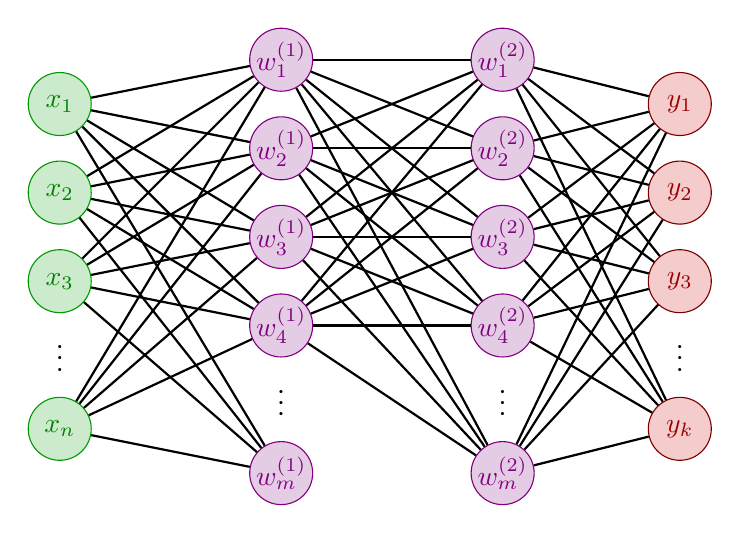
\begin{tikzpicture}[x=1.5cm,y=1.0cm,scale=0.75]

\foreach\i in {1,2,3}
  \node[input]  (x\i)  at (0,-1.5*\i)       {$x_\i$};
\node[input]    (x4)   at (0,-7)            {$x_n$};

\foreach\i in {1,2,3,4}
  \node[hidden] (w_1\i)  at (2.5,0.75-1.5*\i) {$w_\i^{(1)}$};
\node[hidden]   (w_15)   at (2.5,-7.75)       {$w_m^{(1)}$};

\foreach\i in {1,2,3,4}
  \node[hidden] (w_2\i)  at (5.0,0.75-1.5*\i) {$w_\i^{(2)}$};
\node[hidden]   (w_25)   at (5.0,-7.75)       {$w_m^{(2)}$};

\foreach\i in {1,2,3}
  \node[output]  (y\i)  at (7,-1.5*\i)       {$y_\i$};
\node[output]    (y4)   at (7,-7)            {$y_k$};

% connections
\foreach\i in {1,2,3,4,5} \foreach\j in {1,2,3,4}
{
  \draw[black,thick]   (w_1\i) -- (x\j);
  \draw[black,thick]   (w_2\i) -- (w_1\j);
  \draw[black,thick]   (w_2\i) -- (y\j);
}
% dots
\foreach\i/\j in {x3/x4,w_14/w_15,w_24/w_25,y3/y4}
  \node at ($(\i)!0.5!(\j)$) {\strut$\vdots$};
\end{tikzpicture}
\label{fig:neural-network}
\end{figure}

\begin{figure}[tb]
\caption[Common activation functions]{Sigmoid, ReLU, and tanh activation functions.}
\vspace{\baselineskip}
\centering
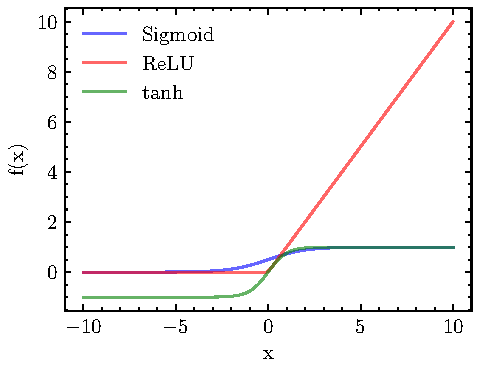
\includegraphics[scale=1.0]{img/sigmoid-relu-tanh}
\label{fig:activation-functions}
\end{figure}

The data feed to an NN is typically divided into two sets. The training dataset is used to train the model by adjusting its parameters based on input samples and corresponding target values. The validation dataset is used to evaluate the model's performance and detect overfitting during training. Overfitting occurs when a model excessively fits the training data but fails to generalize to unseen data.

During training, data can be fed to an NN in batches. A batch refers to a subset of training samples that are processed together during each iteration of an epoch. Instead of updating the weights of the network after processing each individual training sample (which is computationally inefficient), batches allow multiple examples to be processed simultaneously. A larger batch size can lead to more efficient parallel processing but may require more memory. Conversely, a smaller batch size consumes less memory but may result in slower training convergence due to more frequent weight updates.

An epoch is a complete iteration of the entire training dataset. It involves feeding each training sample through the network, updating weights based on the loss function, and performing forward and backward propagation for all training samples. Early stop, also called patience, monitors a metric such as validation loss, and ends the training process if the chosen metric fails to improve for a predefined number of consecutive epochs. Stopping the training early prevents overfitting and improves generalization by preserving the performance of the model at the point of best validation metric.

\begin{definition}[Early Stop]
Let $M$ represent the chosen metric (e.g., validation loss) and $n$ denote the number of consecutive epochs without improvement allowed. Given the current epoch $t$, the training is stopped if the following condition is met:

$$M(t) > \min\{M(t-1), M(t-2), \ldots, M(t-n)\}$$

where $M(t)$ represents the metric value at epoch $t$.
\end{definition}


Standard NNs may suffer from the vanishing gradient problem~\cite{Hochreiter/1991}. The gradients tend to diminish as they propagate backward through multiple layers, making it challenging for earlier layers to learn meaningful representations. This problem hampers the optimization process and restricts the overall performance of the network.

Residual Neural Networks (ResNets)~\cite{He.etal/2016} can reduce the vanishing gradient problem. ResNets use skip connections that bypass layers, allowing the information to flow directly from one layer to another. This bypassing mechanism mitigates the vanishing gradient problem and facilitates the training of deep networks.

\begin{definition}[Skip Connection]
Let us consider a ResNet architecture with $L$ layers. The output of the $l$-th layer is denoted by $a^{l}$, and the output of the previous layer is denoted by $a^{l-1}$. The residual connection between the $l$-th and $l-1$-th layers can be represented as:

$$a^{l} = a^{l-1} + \mathcal{F}(a^{l-1}, W^{l}),$$

where $\mathcal{F}$ represents a residual function, typically implemented as a fully connected layer, and $W^{l}$ denotes the learnable parameters of this function.
\end{definition}

\cref{fig:residual-block} has a visual representation of a small \emph{residual block} with a skip connection.

\begin{figure}[tb]
\caption[A residual block]{A residual block with two hidden layers.}
%\vspace{\baselineskip}
\centering
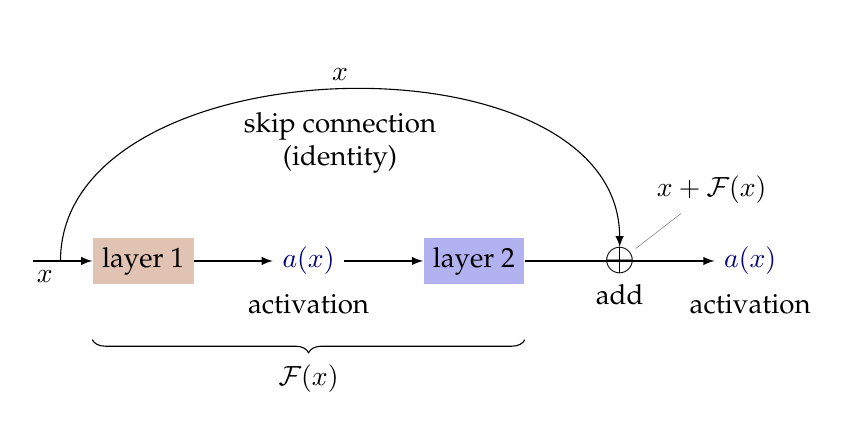
\begin{tikzpicture}[scale=0.70]
  \node[fill=myorange!30] (l1) {layer 1};
  \node[blue!50!black, right=of l1, label={below:activation}] (act1) {$a(x)$};
  \node[fill=myblue!30, right=of act1] (l2) {layer 2};
  \node[right=of l2, font=\Large, label={below:add}, inner sep=0, pin={60:$x + \mathcal F(x)$}] (add) {$\oplus$};
  \node[blue!50!black, right=of add, label={below:activation}] (act2) {$a(x)$};

  \draw[->] (l1) -- (act1);
  \draw[->] (act1) -- (l2);
  \draw[<-] (l1) -- ++(-2,0) node[below, pos=0.8] {$x$};
  \draw[->] (l2) -- (act2) node[above, pos=0.8] {};
  \draw[->] ($(l1)-(1.5,0)$) to[out=90, in=90] node[below=1ex, midway, align=center] {skip connection\\(identity)} node[above, midway] {$x$} (add);
  \draw[decorate, decoration={brace, amplitude=1ex, raise=1cm}] (l2.east) -- node[midway, below=1.2cm] {$\mathcal F(x)$} (l1.west);
\end{tikzpicture}
\label{fig:residual-block}
\end{figure}

\section{Learning Heuristic Functions}
\label{sec:related-h}
While prior research has not specifically addressed learning preferred operators, there have been several studies on using learning heuristic functions for classical planning. These studies can be categorized into two primary approaches.
The first approach heavily relies on domain logic to generate samples and instantiate networks. Its objective is to generalize across domains or a planning formalism.
On the other hand, the second approach minimally uses domain logic solely for generating samples and focuses on generalization within a state space.

The first approach uses structured NNs with architectures specifically designed to align with the characteristics and requirements of the given input task. Examples include learning domain-independent heuristic functions with hypergraph NNs~\cite{Shen.etal/2020}, and learning policies with action schema networks~\cite{Toyer.etal/2018,Toyer.etal/2020} and graph NNs~\cite{Stahlberg.etal/2022}. These approaches are generally applicable to state spaces that differ from the ones they were originally trained on. The major limitation of this set of approaches is that they heavily rely on domain logic, and can also have significant computational overhead, as in the case of action schema networks. Moreover, in domain-independent approaches such as hypergraph NNs, where the network can be applied to a different domain than the one it was originally trained on, the search performance is considerably inferior when compared to logic-based heuristics in terms of coverage. %Furthermore, the major limitation of this set of approaches is that they can not be used to solve planning tasks of the size typically solved by planners as they require excessive memory for instantiation or are too slow in expanding the necessary number of states.

The second approach uses supervised learning to train a feedforward NN with pairs of states and cost-to-goal estimates. Samples can be generated with forward search from the initial state~\cite{Ferber.etal/2020a}, backward search from the goal~\cite{Yu.etal/2020,OToole/2022,Bettker.etal/2022}, or a combination of both~\cite{Ferber.etal/2022}.
This set of approaches offers the advantage of requiring less computational resources than the first set. However, a limitation is that the trained models are typically applicable only within the specific state space they were trained on. Search performance is also a problem, since these approached typically solve less tasks than simple logic-based heuristics such as goal-count. An advantage is that this set of approached rely on domain logic to a lesser extent, and only during sample generation, such as determining applicable operators and mutexes. Moreover, in cases where a generator of predecessor and successor states is available, which can also be learned, these approaches can eliminate the requirement for domain-specific logic.%\pp{Not really, since partial states.}

%In this context,~\citet{Ferber.etal/2020a} conducted a systematic study on the hyperparameters of the feedforward NN architecture and found that their influence is secondary. They discovered that, for a fixed architecture, two main factors significantly impact the informativeness of the heuristic: the selection of the sample subset and the size of the sample set.

%Some approaches sample states by backward searches from the goal~\cite{Yu.etal/2020, OToole/2022, Bettker.etal/2022}.
Regarding sampling by backward search,~\citet{Yu.etal/2020} used depth-first search,~\citet{OToole/2022} used random walks, and~\citet{Bettker.etal/2022} used a combination of breadth-first search and random walks. In these cases, the cost-to-goal estimates were assigned as the lowest distance from the goal at which the states were generated.~\citet{Ferber.etal/2022} used a combination of backward and forward searches, using bootstrap learning~\cite{Arfaee.etal/2011}.
Specifically,~\citet{Bettker.etal/2022} introduce several cost-to-goal improvement methods to enhance sample quality and emphasize that the effectiveness of learned heuristics relies on two crucial factors: a sample set that encompasses diverse regions of the state space and accurate cost-to-goal estimates; one without the other is insufficient.

This work follows the second set of approaches, and we generate samples by backward search.
%$To concurrently generate samples and learn a heuristic function,~\citet{Ferber.etal/2022} employed a bootstrapping method~\cite{Arfaee.etal/2011}, where initially new initial states are generated using backward random walks, which are then solved using GBFS guided by the learned heuristic. The resulting plans yield samples, with each sample corresponding to a state within the plan and its associated cost-to-goal estimate. These samples are subsequently used to further train the neural network, aiming to enhance the learned heuristic.

% O'Toole (2022) also presented a method for generating samples that does not involve expansions. This method includes randomly generating states with high cost-to-goal estimates and including them in the sample set. O'Toole demonstrated that this approach substantially increases coverage.



%
% - - - - - - - - - - - - - - - -- - - - - -
% sample generation
% - - - - - - - - - - - - - - - -- - - - - -
% now we talk about the stuff we're doing
%
\chapter{Sample Generation}
\label{cha:sample-gen}
This chapter presents the methods we use to generate samples for training, specifically to train an NN that predicts $h$-values (\cref{sec:sample-learn-h}), and another to train an NN that identifies preferred operators (\cref{sec:sample-learn-po}).

There are multiple techniques available to generate a sample set for training NNs in planning. These techniques include search methods like breadth-first search (BFS), depth-first search (DFS), and random walk (RW). In search methods, the generation of the sample set typically begins from a source node, which is commonly the initial state for forward search or the goal state for backward search (regression). Random sampling of the state space can also be used to generate the sample set. Unlike search methods, random sampling produces independent samples, as each state is generated without relying on previous samples. Sample distribution influences NN generalization~\cite{Ferber.etal/2020a}, and this influence varies depending on the choice of sampling algorithm~\cite{Bettker.etal/2022}.

\section{Sampling for Learning Heuristic Functions}
\label{sec:sample-learn-h}
To learn heuristic functions, states are labeled with a cost-to-goal estimate during sampling. In regression-based methods, the value assigned to a sampled state is determined by its distance to the goal. To generate samples, we use regression to expand the BSS. Specifically, we follow the best-performing approach used by~\citet{Bettker.etal/2022}, using a combination of BFS with multiple rollouts RW, named \bfsrw, which aims to achieve good coverage near the goal (\bfs) while obtaining a diverse set of samples from the remaining state space (\rw).

A regression rollout refers to a sequence of partial state expansions, which concludes under two conditions: either when the last expanded state has no predecessors or when it reaches the depth limit $L$. The process of generating samples halts once the desired number of samples $N$ has been attained. Random walks can have multiple rollouts due to the depth limit $L$, whereas BFS has a single rollout. Repeated states are discarded during each RW rollout to avoid cycles during backward search. However, repeated states are permitted between rollouts.
\citet{Bettker.etal/2022} set the regression limit to $L=\ceil{\facts/\overline{\eff}}$ where $\overline{\eff}=\sum_{o\in \mathcal{O}} |\eff(o)|/|\mathcal{O}|$, i.e.,~the number of facts per mean number of effects in the operators of the input task. Unlike using a fixed $L$~\cite{Yu.etal/2020, OToole/2022}, this adaptive $L$ aims to approximate the longest distance $d^{*}$ between the goal state and any potential initial state.
% However, if the backward state space contains an insufficient number of states to generate the required $N$ samples, BFS may need to perform multiple rollouts.

\bfsrw consists of two phases. In the first phase, a fixed percentage $p_\bfsrw$ of the $N$ samples is generated using BFS. The BFS expands a state from layer $k$ and generates $n$ states from layer $k+1$. These generated states are sampled only when $N + n \leq p_{\bfsrw}N$, otherwise, no states are sampled, and BFS expands another state. The set of unexpanded states, i.e., leaves, is denoted as $Q$. The second phase involves multiple random walk rollouts starting from randomly selected states in $Q$. This process continues until the sample set reaches $N$. During the random walk phase, states already sampled in the BFS phase are not sampled again.

After finishing regression,~\citet{Bettker.etal/2022} improve the cost-to-goal estimates of each sampled partial state~(\cref{sec:sample-improving-h}), and complete them to full states~(\cref{sec:sample-completion}).~\ppi{Note that I don't mention randomly generated samples here, only a small remark in the Experiments section. I don't think they're useful for POs and are far more important in Rafael's dissertation.}

%\begin{algorithm}
%\caption{Sampling states for heuristic values using \bfsrw}
%\begin{algorithmic}[1]
%\Procedure{\bfsrw}{$\Pi$, $N$, $L$, $p_\bfsrw$}
%\State \textbf{Phase 1}
%\State Initialize empty set $Q$
%\State Initialize empty set $S_{bfs}$
%\State $S_{bfs}$, $Q \gets$ BFSLimited($s_{0}$, $p_{\bfsrw}N$)
%
%\State Initialize empty set $S_{rw}$
%\State \textbf{Phase 2}
%\State Initialize Boolean array $V$ of size $|Q|$ with all indexes set to $False$
%\While{$|S| < N$}
%    \State $rnd\_idx \gets$ random index of $Q$ where  $V$[$rnd\_idx$]$ = False$
%    \State $V$[$rnd\_idx$]$~\gets True$
%    \If{all positions in $V$ are $True$}
%      \State Set all positions in $V$ to $False$~\emph{\# ``Replacement''}
%    \EndIf
%    \State Initialize a partial state $s$
%    \State $s \gets$ $Q$[$rnd\_idx$]
%    \State $n_{rw} \gets min(L - h(s), N - |S|)$ \# \emph{$n$ states to sample in this RW rollout}
%    \State $S_{rw} \gets$ RW($s$, $n_{rw}$) \# \emph{Random walk sampling starting from $s$}
%    \State $S \gets S \cup (S_{rw} \setminus S_{bfs}) $
%\EndWhile
%\State \textbf{return} $S$
%\EndProcedure
%\end{algorithmic}
%\end{algorithm}

%\begin{algorithm}
%\caption{Breadth-first search of \bfsrw}
%\begin{algorithmic}[1]
%\Procedure{BFSLimited}{$s_{0}$, $M$}
%\State Initialize set $Q$ with $s_{0}$
%\State Initialize set $K$ with $s_{0}$ \emph{\# i.e., layer $k$}
%\State Initialize empty set $K_{+1}$ \emph{\# i.e., layer $k+1$}
%\State Initialize set $S_{bfs}$ with $s_{0}$
%\While{$|S_{bfs}| < M$ and $K$ is not empty}
%    \State Shuffle $K$
%    \ForAll{partial states $s$ of $K$}
%      \State Initialize empty set $P_{s}$
%      \State $P_{s} \gets \{s' \mid s' \in pred_{bfs}(s)~\text{and}~s' \notin S_{bfs}\}$
%      \If{$|S_{bfs}| + |P_{s}| \le  M$}
%          \State $S_{bfs} \gets S_{bfs} \cup P_{s} $
%          \State $K_{+1} \gets K_{+1} \cup P_{s} $
%          \State $Q \gets (Q \cup P_{s}) \setminus \{s\} $
%      \EndIf
%      \If{$|S_{bfs}| = M$}
%        \State break
%      \EndIf
%    \EndFor
%    \State $K \gets K_{+1}$
%    \State $K_{+1} \gets \emptyset$
%\EndWhile
%\State \textbf{return} $S_{bfs}$, $Q$
%\EndProcedure
%\end{algorithmic}
%\end{algorithm}

%\section{Maximum Regression Limit}
%\label{sec:sample-maximum-regression-limit}
%In previous work by \citet{Yu.etal/2020} and \citet{OToole/2022}, a maximum limit $L$ of $200$ and $500$, respectively, has been used to restrict expansion depth. However, using a fixed limit may not be the optimal choice for tasks with state spaces of varying diameters or different maximum distances to a fixed goal when seeking a representative sample of the state space. This becomes particularly problematic in regression, as an overestimated maximum regression limit $L$ can result in inflated cost-to-goal estimates, while an underestimated limit can lead to an excessive concentration of samples near the goal.
%
%Hence, it is essential to determine the optimal maximum regression limit for a fixed goal as a function of the longest distance \distfarthest between the goal state and any potential initial state. While BFS can provide an accurate estimate of \distfarthest, DFS and random walks need higher limits due to their tendency to deviate from the shortest paths. Since the exact value of \distfarthest is typically unknown, we propose an adaptive and approximated approach to define the maximum regression limit $L$ based on the input task parameters. This adaptive method allows us to tailor the limit according to the specific characteristics of the task.
%Thus, we set the regression limit to $L=\ceil{\facts/\overline{\eff}}$ where $\overline{\eff}=\sum_{o\in \mathcal{O}} |\eff(o)|/|\mathcal{O}|$, i.e.,~the number of facts per mean number of effects in the operators.

\section{Improving Cost-to-Goal Estimates}
\label{sec:sample-improving-h}
%\citet{Bettker.etal/2022} also developed two methods to improve the cost-to-goal estimates of each sampled state.
%Let us begin by noting that cost-to-goal estimates always provide a lower bound on the true cost-to-goal $h^{*}$, as explained below.

%\begin{property}
%\label{prop:hvalue}
%The cost-to-goal estimate $h(s)$ of a sample $s$ obtained by regression satisfies $h(s)\geq h^*(s)$.
%\end{property}

%\begin{proof}
%This follows because each estimate is witnessed by a plan.
%A valid regression sequence $\rho=(o_1,\ldots,o_k)$ produces a series of partial states that can reach the goal within a maximum of $k$ steps and with a cost no greater than $\sum_{i\in[k]}\text{cost}(o_i)$. The cost of this sequence cannot be lower than the optimal cost.
%\end{proof}

Better $h$-value estimates generally result in improved learned heuristics, leading to fewer expanded states during a search. However, this correlation is not always guaranteed~\cite{Holte/2010}. To enhance the cost-to-goal estimates of each sampled state,~\citet{Bettker.etal/2022} developed two methods that are used in this study. The first method, called \sai, minimizes estimates across repeated samples, while the second method, named \sui, minimizes estimates across the successors of samples.


\subsection{Sample Improvement}
\label{sec:sample-sai}
It is possible to generate duplicate states with different estimates due to multiple random walk rollouts. Thus, we update the cost-to-goal estimate for each sampled state $s$ to the minimum estimate $h(s) = \min\{h_i \mid s=s_i, i\in[N]\}$.
% This update is applied to both partial and complete states since identical complete states can be generated from different partial states.
This procedure is called ``sample improvement'' (\sai).

\subsection{Successor Improvement}
\label{sec:sample-sui}
In addition to sampling the same states, it is common to sample neighboring states in the state space, especially for states close to the goal. We can leverage this to enhance the cost-to-goal estimates using the following approach, starting by constructing a graph $G$ containing the relations between all states in the sample set.
%Let $G=(V,A)$ be a directed graph representing all sampled partial states, where~$V=\{s_i\mid i\in[N]\}$. For every pair of states $s$ and $t$ in $V$, if there exists an operator $o\in\mathcal{O}$ applicable to $s$ such that $\sucs(s,o)\subseteq t$, we add an arc $(s,t)$ of length $\text{cost}(o)$ to $A$. Note that, unlike in regression, if $\pre(o)$ mentions to an undefined variable in $s$, then $o$ is not applicable.
%
\begin{definition}[Sample Set Graph]\label{def:graph}
A sample set graph is a directed and labeled graph~$G = (V, A)$ defined by the states obtained in the sampling. Each vertex is labeled by a sampled partial state, i.e., $V = \{s_i \mid i \in [N]\}$. (Note that the undefined variables of a partial state can typically be completed in multiple ways, so each vertex represents a set of complete states.) Set $A$ contains an arc $(s,t)$ for each operator $o \in \mathcal{O}$ where $\sucs(s,o) \subseteq t$, i.e., $\sucs(s,o)$ can become $t$ from an assignment of undefined variables.
\end{definition}

To efficiently manage subsets, we use a trie data structure to store all the samples and search for successors in states that are supersets. When dealing with partial states generated by regression, we can always find at least one successor, except for the goal state $s^{*}$. We proceed by computing the shortest paths to the goal in the graph $G$ using Dijkstra's algorithm. Subsequently, we update the cost-to-goal estimates of each state accordingly. This process is called ``successor improvement'' (\sui).


\section{Sample Completion}
\label{sec:sample-completion}

Regression sampling generates a set of partial states with undefined variables. However, during the search, the NN is trained on and expects complete states as input.
Each partial state can be completed by assigning a value $s(v)\in\dom(v)$ to all fact pairs $(v,s(v))$ where $s(v)=\bot$.
To complete partial states, we use a method that assigns a random value $s(v) \in \dom(v)$ to each undefined variable. However, we ensure that the assigned values satisfy mutexes derived from the planning task. We process the undefined variables in a random order and assign them random values that do not violate the mutexes. If, after $10$\,K attempts, we are unable to complete the state, we leave the corresponding facts undefined, setting them to false.%\footnote{In practice, this situation is extremely rare, occurring in only about $0.1\,\%$ of the samples.}


\section{Ideal Preferred Operators}
\label{sec:sample-ideal-po}
Ideally, we want preferred operators that help solve a task with the least effort, which we call ideal preferred operators.

\begin{definition}[Ideal Preferred Operator]\label{def:ideal_preferred_operator}
  An ideal preferred operator generates a state with the shortest distance to the goal among all successors. Given a state $s$ and an operator~$o \in \mathcal{O}$ where $\sucs(s,o) = t$, $o$ is an ideal preferred operator if $\hstarp{t} = \min_{s' \in \sucs(s)} \hstarp{s'}$.
\end{definition}

Every state $s$ that has a plan is associated with at least one preferred operator. These preferred operators generate successor states $t$ where $\hstarp{t} < \hstarp{s}$. Thus, only the goal states and dead-end states lack preferred operators.
\ppi{Removed the property and the proof for now.}
%\begin{property}
%  \label{prop:ideal-optimal}
%  GBFS only expands states on an optimal path if using a safe heuristic function, ideal preferred operators, tie-breaking by larger g-value, and starting with infinite boost (only states from the preferred queue are expanded during search).
%\end{property}

%\begin{proof}
%We will prove the property by contradiction.
%
%Suppose a state $s$ expanded by GBFS from the preferred queue is not on any optimal path.
%Let $\pi^*$ be an optimal path from the initial state $s_0$ to the goal state $s^*$. Since $s$ is not on any optimal path, there must be another path $\pi = s_0,\ldots,s,\ldots,s^*$ greater than $\pi^*$.
%Let $s'$ be the last state on the optimal path $\pi^*$ before diverging to $\pi$, and let $s''$ be the next state on $\pi$ after diverging from $\pi^*$, i.e., $s''$ is a successor of $s'$. Note that $h^*(s') < h^*(s'')$ because a lower $h$-value determines an optimal path.
%
%Now, consider the situation when the search reaches $s'$ during the expansion process. At this point, $s'$ has already been expanded, and all its successors have been generated. Since $s'$ is on the optimal path, the ideal preferred operator used to generate $s''$ must have the property that $h^*(s'') = \min_{t \in \sucs(s')} h^*{(t)}$. However, we have already established that $h^*(s') < h^*(s'')$. This contradicts the definition of an ideal preferred operator, as the operator used to generate $s''$ should have the smallest $h^*$ value among all successors of $s'$. Therefore, our assumption that there exists a state not on the optimal path expanded by GBFS is false.

%Since GBFS expands states in a best-first manner using ideal preferred operators, tie-breaking by larger g-value, and infinite boosting where the first expansion is a state generated by preferred operators (meaning that only states generated by preferred operators are expanded), it only explores successors with the lowest $h^*$ values. As the optimal path consists of states with the lowest $h^*$ values, GBFS will expand states only on the optimal path, ultimately reaching the goal state.

%\end{proof}

\section{Discovered Preferred Operators}
\label{sec:sample-discovered-po}
Obtaining ideal preferred operators is challenging for large tasks as we lack access to the complete search state space, and computing the \hstar-values for all states may be intractable. To address this, we compute the preferred operators within a sample set of the state space, without relying on \hstar-values. We construct a sample set graph $G$~(\vref{def:graph}) by mapping operators that transition between two samples and then determine the operators that contribute to the shortest path to the goal.

In the graph $G$, each arc represents an applicable operator between two sampled states. Every sample, except for the goal states, has at least one successor, so it is feasible to trace multiple paths from a sampled state to a goal state. By selecting the operators associated with the shortest path, we can identify the preferred operators for reaching a goal state.

\begin{definition}[Discovered Preferred Operators]\label{def:discovered_preferred_operators}
Let $G = (V, A)$ be the sample set graph and $G' = (V, A')$ be the shortest path sample set graph. We run Dijkstra's algorithm on $G$ to find the shortest path to each vertex $v \in V$. Every arc of $A$ that has a shortest path of at least one vertex $v$ is inserted in $A'$. The discovered preferred operators of the set of states $s$ (since $s$ is a partial state with undefined variables) are the operators represented by the outgoing arcs $a \in A'$ of the vertex labeled by $s$.
\end{definition}

The quality of the discovered preferred operators depend on the quality of the shortest paths. The quality of these paths, in turn, relies on the accuracy of the $h$-values assigned to each sampled state.
Furthermore, a state can have multiple discovered preferred operators if it has multiple shortest paths. \cref{fig:spg-example} has an example of a sample set graph $G$ with two shortest paths from the partial state $s_{1}$ to the goal $s^{*}$. The preferred operators of $s_{1}$ are thus $\{o_{2}, o_{3}\}$.

\begin{figure}[tb]
\caption[Example sample set graph with two shortest paths]{Example samplet set graph with two shortest paths (red, orange) from $s_{1}$ to the goal $s^{*}$.}
\centering
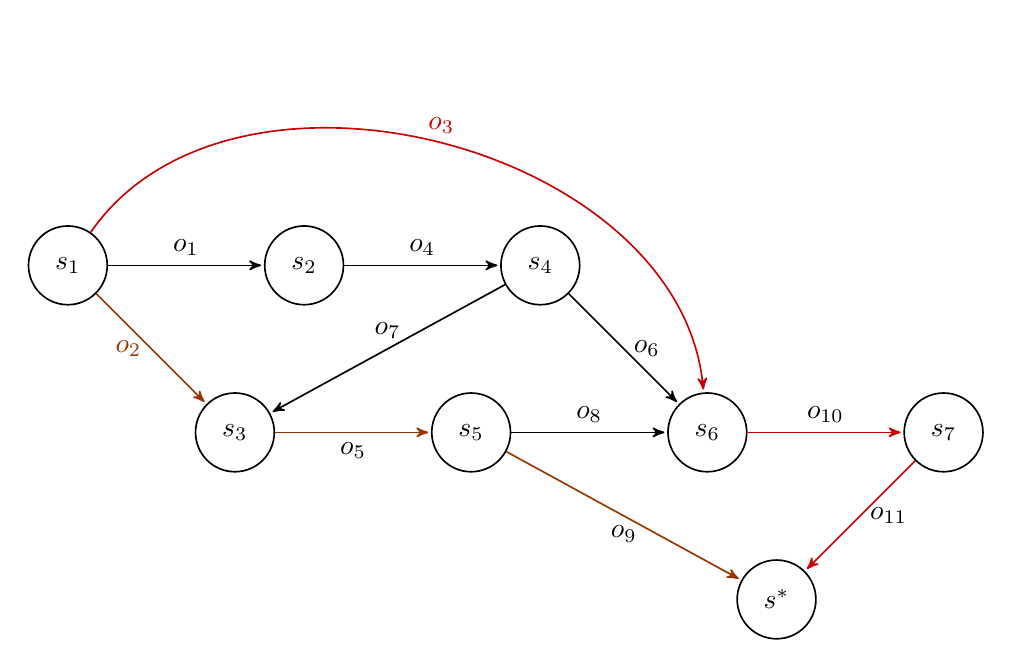
\begin{tikzpicture}[->,>=stealth',shorten >=1pt,auto,node distance=3cm,semithick]
  \tikzstyle{state}=[circle,draw,minimum size=1cm]

  \node[state] (s1) {$s_1$};
  \node[state] (s2) [right of=s1] {$s_2$};
  \node[state] (s3) [below right of=s1] {$s_3$};
  \node[state] (s4) [right of=s2] {$s_4$};
  \node[state] (s5) [right of=s3] {$s_5$};
  \node[state] (s6) [below right of=s4] {$s_6$};
  \node[state] (s7) [right of=s6] {$s_7$};
  \node[state] (s8) [below left of=s7] {$s^*$};

  \path (s1) edge node[above] {$o_{1}$} (s2);
  \path [->, color=myorange] (s1) edge node[left] {$o_{2}$} (s3);
  \path [->, color=myred] (s1) edge [bend left=70] node[above] {$o_{3}$} (s6);
  \path (s2) edge node[above] {$o_{4}$} (s4);
  \path (s3) edge [draw=myorange] node[below] {$o_{5}$} (s5);
  \path (s4) edge node[right] {$o_{6}$} (s6);
  \path (s4) edge node[above] {$o_{7}$} (s3);
  \path (s5) edge node[above] {$o_{8}$} (s6);
  \path (s5) edge [draw=myorange] node[below] {$o_{9}$} (s8);
  \path (s6) edge [draw=myred] node[above] {$o_{10}$} (s7);
  \path (s7) edge [draw=myred] node[right] {$o_{11}$} (s8);
\end{tikzpicture}
\label{fig:spg-example}
\end{figure}

\section{Sampling for Learning Preferred Operators}
\label{sec:sample-learn-po}
The sample generation approach described in~\cref{sec:sample-learn-h} is not suitable for learning preferred operators due to the presence of duplicate samples within rollouts. This leads to a sample set that contains numerous repeated samples, which offer no additional value when constructing the shortest path graph $G'$ for identifying preferred operators. Consequently, this approach fails to effectively explore the state space and identify additional preferred operators. To address this limitation, we have developed an alternative sample generation method specifically designed to discover preferred operators, dubbed~\bfsrs, divided into two phases.

Let $S_1$ and $S_2$ denote the sets of samples generated in the first and second phases of~\bfsrs, respectively. The complete sample set is represented by $S = S_1 \cup S_2$, consisting of $N$ distinct samples. Let $k_1$ and $k_2$ be variables satisfying $k_1 + k_{2} = 1$.
In the first phase of the algorithm, we use BFS by applying backward applicable operators from the goal state until expanding $k_1N$ states, which are then added to $S_1$.
In the second phase, we maintain two queues first initialized during BFS: an open queue, containing states generated but not yet expanded, and a closed queue, comprising states that have been expanded and already sampled. During each iteration, we randomly select a state from the open queue, move it to the closed queue, add it to the sample set $S_2$, and insert its predecessors into the open queue if they are not already present in either queue. The sampling process continues until $|S_2| = k_2N$.
See \cref{alg:sampling-po}. The primary distinction between phases one and two is the selection process for expanding states from the open queue. Unlike phase one, where the first-in, first-out approach of BFS is used, phase two involves randomly selecting a state from the open queue for expansion. We do not use a regression limit $L$ as in \bfsrw, but in practice our maximum regression depth remained close to $d^{*}$.
%Note that this algorithm has a single rollout, so no maximum regression limit $L$ is used.
%See \cref{alg:sampling-po,alg:sampling-bfs}. Note that this algorithm has a single rollout, so no maximum regression limit $L$ is used.

\begin{algorithm}[tb]
\caption{Sampling states for preferred operators using \bfsrs}
\label{alg:sampling-po}
\begin{algorithmic}[1]
\Procedure{BRS}{$s^{*}$, $N$, $k_{1}$, $k_{2}$}
  \State $open = \emptyset$
  \State $S_{1} = \emptyset$
  \State \textcolor{gray}{\# Phase 1: populates $S_{1}$ and $open$ with BFS.}
  \State $S_{1}, open \gets$ BFS($s^{*}$, $open$, $k_1N$)
  \State $closed = S_{1}$
  \State \textcolor{gray}{\# Phase 2: populates $S_{2}$ with random elements $s$ from $open$.}
  \State $S_{2} = \emptyset$
  \While{$|S_{2}| < k_{2}N$}
    \If{$open =  \emptyset$}
      \State \textbf{return} $S_{1} \cup S_{2}$ (backward state space fully explored)
    \EndIf

    \State $i \gets$ random index of $open$
    \State \textcolor{gray}{\# Initialize a partial state $s$.}
    \State $s \gets$ $open$[$i$]
    \State Remove element at $open$[$i$]
    \State $closed \gets closed \cup \{s\}$
    \State $S_{2} \gets S_{2} \cup \{s\}$
    \State $P \gets \{s' \mid s' \in pred(s)\}$
    \ForAll{partial states $s' \in P$}
      \If{$s' \notin (open \cup closed)$}
        \State Insert $s'$ into $open$
      \EndIf
    \EndFor
  \EndWhile

  \State \textbf{return} $S_{1} \cup S_{2}$
\EndProcedure
\end{algorithmic}
\end{algorithm}

%\begin{algorithm}[tb]
%\caption{Breadth-first search of \bfsrs}
%\label{alg:sampling-bfs}
%\begin{algorithmic}[1]
%\Procedure{BFS}{$s^{*}$, $open$, $M$}
%  \State $S_{1} = \emptyset$
%  \State $open \gets open \cup \{s^{*}\}$
%
%  \While{$|S_{1}| < M$}
%    \If{$open =  \emptyset$}
%      \State \textbf{return} $S_{1}$ (backward state space fully explored)
%    \EndIf
%    \State \textcolor{gray}{\# Initialize a partial state $s$}
%    \State $s \gets$ first element in $open$
%    \State Remove first element in $open$
%    \State $S_{1} \gets S_{1} \cup \{s\}$
%    \State $P \gets \{s' \mid s' \in pred_{bfs}(s)\}$
%    \ForAll{partial state $s' \in P$}
%      \If{$s' \notin open$}
%        \State $open \gets open \cup \{s'\}$
%      \EndIf
%    \EndFor
%  \EndWhile
%
%  \State \textbf{return} $S_{1}$
%\EndProcedure
%\end{algorithmic}
%\end{algorithm}

We apply \sai and \sui and complete the states as described in~\cref{sec:sample-improving-h,sec:sample-completion}.

%\section{Randomly Generated Samples}
%\label{sec:sample-random-samples}
%\citet{OToole/2022} demonstrated that augmenting a sample set generated through expansion with randomly generated samples enhances the performance of the search algorithm guided by the learned heuristic. They suggest assigning a cost-to-goal estimate of $L+1$ to randomly generated samples, where $L$ represents the maximum regression limit.
%The samples are generated from undefined states and are completed as discussed in~\cref{sec:sample-completion}. If the generated state $s$ is already present in the sample set, denoted as $s = s_i$ for some $i\in[N]$, it is assigned the cost-to-goal estimate $h_i$. Conversely, if the state $s$ is not already in the sample set, it is given a cost-to-goal estimate of $1+\max_{i\in[N]} h_i$, ensuring that the estimate is larger than all existing estimates.

%
% - - - - - - - - - - - - - - - -- - - - - -
% experiments
% - - - - - - - - - - - - - - - -- - - - - -
% empiricism!
%
\chapter{Experiments}
\label{cha:exp-experiments}
This section presents four of experiments. In the first (\cref{sec:exp-learning-po}), we investigate learning preferred operators and establish an upper-bound performance measure using the ideal preferred operators~\postar. The second experiment (\cref{sec:exp-performance-po}) evaluates learning discovered preferred operators~\pog from sample sets of varying sizes and compares them to logic-based preferred operators. The third experiment (\cref{sec:exp-comparison-sample-method}) compares the results with preferred operators learned from a sample set generated using two distinct sampling methods, as described in~\cref{sec:sample-learn-h} and~\cref{sec:sample-learn-po}. Finally, in the fourth experiment~(\cref{sec:other-heuristic-functions}), we analyze the learned preferred operators~\pog in conjunction with several logic-based heuristic functions.

\section{Configuration}
\label{sec:exp-configuration}
We use the same network architecture as \citet{Ferber.etal/2022},~\citet{OToole/2022}, and~\citet{Bettker.etal/2022} with modifications to support learning preferred operators. Specifically, we use a ResNet with He initialization~\cite{He.etal/2015}, consisting of two hidden layers followed by a residual block containing two hidden layers.
Each hidden layer has $250$ neurons and is ReLU-activated.
The training uses the Adam optimizer~\cite{Kingma.Ba/2015} with a learning rate of $10^{-4}$, a batch size of $64$, and an early stop patience\pp{Patience is now explained in the background.} of $100$ epochs.
We use the MSE loss function to learn heuristic values in a regression context, and for learning preferred operators we opt for the BCE loss since learning preferred operators is a multi-label classification problem.
The input of the NN consists of samples in the format $(h(s), \mathcal{F}(s), O_{pref} \subseteq O)$
where $\mathcal{F}(s)$ is a Boolean representation of the input state $s$, with $0$ if a proposition is false and $1$ otherwise~(\cref{sec:background-heuristics}), $h(s)$ is the target value in the regression network representing the $h$-value for $s$, and $O_{pref}$ are the target values in the classification network representing the preferred operators for state $s$.

The output for the regression network is a single ReLU-activated neuron representing the learned $h$-value, and the output for classification is a sigmoid-activated tensor with values in the range $[0, 1]$ and a size equal to the number of operators of the input task.
Each output neuron corresponds to an indexed operator. For example, in a planning task with ten operators, in which a sampled state $s$ has target preferred operators of indexes two and five, the indexes two and five of the output tensor of size ten must be maximized~(\cref{fig:po-tensor}). The training set has $90\,\%$ of the data, while the validation set contains the remaining $10\,\%$.

\begin{figure}[tb]
\caption[]{Example tensor with two preferred operators as target values.}
\vspace{\baselineskip}
\centering
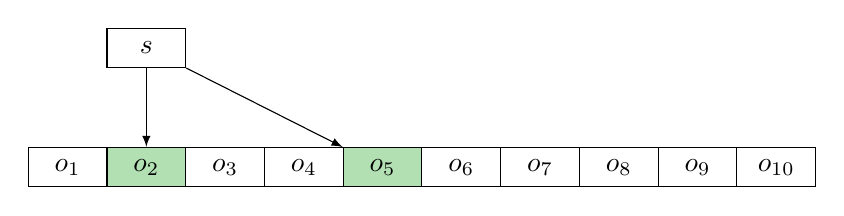
\begin{tikzpicture}[node distance=1cm]
  % Operators
  %\foreach \x in {1,...,10}
  %  \node[draw, minimum width=1cm, minimum height=0.5cm] (op\x) at (\x,0) {$o_{\x}$};
  \foreach \x in {1,...,10}{
    \ifnum\x=2
      \node[draw, minimum width=1cm, minimum height=0.5cm, fill=mygreen!30] (op\x) at (\x,0) {$o_{\x}$};
    \else
      \ifnum\x=5
        \node[draw, minimum width=1cm, minimum height=0.5cm, fill=mygreen!30] (op\x) at (\x,0) {$o_{\x}$};
      \else
        \node[draw, minimum width=1cm, minimum height=0.5cm] (op\x) at (\x,0) {$o_{\x}$};
      \fi
    \fi
  }
  % Sampled state
  \node[draw, minimum width=1cm, minimum height=0.5cm, above=of op2] (s) {$s$};

  % Arrows
  \draw[->] (s) -- (op2);
  \draw[->] (s) -- (op5);
\end{tikzpicture}
\label{fig:po-tensor}
\end{figure}


%\subsection{Neural Network Initialization}
%\label{sec:exp-nn-init}
%While training NNs, a phenomenon known as ``born dead'' as described by~\citet{Lu.etal/2020}, can occur when the network outputs zero for all training samples after initialization. We observed this phenomenon happens frequently in experiments involving learning heuristic functions on smaller state spaces with fewer samples. To address this, we implemented a test to check if the network outputs zero for all training samples after initialization. If this condition is met, we reinitialize the network with a different seed until it produces a non-zero output for at least one sample.

\subsection{Extracting Preferred Operators}
\label{sec:exp-extracting-pos}
We extract the predicted preferred operators from the NN by selecting the operator with the highest output value. Additionally, if there are any operators with output values greater than $0.9$, we include them in the selection. We do this to avoid false positives since most tasks considered in this work have a mean number of preferred operators close to one. Through experimentation, we found that this strategy produced better results than selecting only operators with output values above an arbitrary threshold, as lowering the threshold resulted in poorer performance.

\subsection{Dataset}
\label{sec:exp-dataset}
Our dataset consists of planning tasks with state spaces ranging from $40$\,K to $1$\,M states, which is identical to the dataset used by~\citet{Bettker.etal/2022}. To generate samples, we use one task in each of the following domains: Blocks World (abbreviated as Blocks), Grid, N-Puzzle, Rovers, Scanalyzer, Transport, and VisitAll. \cref{tab:tasks_info} has relevant information regarding each task, and~\vref{cha:tasks_each_domain} contains a small description of each domain. The output neurons in the classification NN correspond to the number of operators, whereas the regression NN used for learning heuristics produces a single numerical value as its output. The input neurons are determined by the number of facts.


We evaluate the results based on the number of expanded states since all planning tasks are solved. Each FSS has $50$ randomly generated initial states, resulting in $50$ planning tasks. %We generate these initial states by conducting a random walk of length $200$ from the original initial state of a task. However, in the Rovers, Scanalyzer, and VisitAll domains, some initial states were duplicated or already satisfied the goal state. As a result, we generate initial states for these domains using random walks of length $25$, $50$, and $8$, respectively.
In the tables, each cell represents the mean value across $50$ planning tasks and $25$ seeds, i.e., $5$ sample seeds $\times$ $5$ network seeds. Each sample seed represents a different set of samples, while the network seeds are used to initialize the parameters of NN.
Additionally, when referring to a specific number of samples, we use the notation ``$n$ percent of the state space'' to denote a fraction of the FSS, e.g., $5\,\%$ of Block World's FSS is $\lfloor 65990 \times 0.05 \rceil = 3300$ samples.

\begin{table}[htb]
\centering
\caption{Information on the task used for each domain. The forward state space size, the distance \distfarthest of the state most distant from the goal state, regression limit $L$, the number of facts, and the number of operators.}
\vspace{\baselineskip}
\begin{tabular}{lrrrrr}
\toprule
Domain     & FSS size & \distfarthest & $L$  & \# facts & \# operators \\ \midrule
Blocks     & 65990    & 24            & 17   & 64       & 98           \\
Grid       & 452353   & 32            & 44   & 76       & 252          \\
N-Puzzle   & 181440   & 31            & 41   & 81       & 192          \\
Rovers     & 565824   & 19            & 27   & 32       & 57           \\
Scanalyzer & 46080    & 15            & 20   & 42       & 300          \\
Transport  & 637632   & 17            & 35   & 66       & 572          \\
VisitAll   & 79931    & 15            & 17   & 31       & 48           \\ \bottomrule
\end{tabular}
\label{tab:tasks_info}
\end{table}


\subsection{Training}
\label{sec:exp-training}
Sample generation is implemented in Neural Fast Downward~\cite{Ferber.etal/2020a}, and we use PyTorch 1.9.0~\cite{Paszke/2019} for defining and training the NNs. The experiments were conducted on Ubuntu~$20.04$~LTS~GNU/Linux machines with an AMD~Ryzen~$9$~$3900$X $12$-core processor ($4.2$~GHz) with a memory limit of $4$~GB and one core per process. The NNs were trained until convergence, with the most complex networks requiring approximately two hours of training~(see \cref{tab:training_info} in the appendix).

\subsection{Evaluation}
\label{sec:exp-evaluation}
We use Fast Downward~\cite{Helmert/2006} with GBFS to solve all $50$ initial states of each domain using a heuristic with the learned preferred operators and a $5$ minute search time limit for each planning task.
When preferred operators are considered, we experimented with searches using dual-queues with and without boosting. Due to better experimental results, for the following experiments we use a boosted dual-queue with a boosting value of $1000$, as in~\citet{Richter.Helmert/2009}. Results for searches with boosting disabled are available in~\vref{cha:discovered_pos_boost0}.

\subsection{Sampling}
\label{sec:exp-sampling}
We obtain the learned heuristic \hnn by training over samples generated as described in~\cref{sec:sample-learn-h}, with the best configuration from~\citet{Bettker.etal/2022}, i.e., sample set size equal to $1\,\%$ of the state space, regression limit of $L=\ceil{\facts/\overline{\eff}}$, and setting $p_{\bfsrw}=10\,\%$ of the total number of samples. We also add a quantity of randomly generated samples equal to $20\,\%$ of the total number of samples, with cost-to-goal estimates equal to the maximum estimate of the existing samples obtained through regression plus one.

Since in this work we are only interested in the effects of learned preferred operators, the learned heuristic functions \hnn for each task have the fixed configuration described above. To obtain the learned preferred operators \pog, we train the NNs over sample sets generated according to the method described in~\cref{sec:sample-learn-po}, with $k_1 = 0.1$ and $k_2 = 0.9$. \pp{We actually don't have evidence of why we used 0.1 and 0.9. They're leftovers from the previous method, FSM.}

\section{Learning Preferred Operators}
\label{sec:exp-learning-po}
% Clear, objective description of this section
This section compares task-solving performance with and without preferred operators using several configurations: \hstar, which represents the perfect heuristic; \hnn, which is a learned heuristic without preferred operators; \postartable, an oracle of ideal preferred operators; \postar, learned ideal preferred operators; \pogstar, discovered preferred operators using \hstar for shortest path distance calculation; and \pog, discovered preferred operators using Dijkstra's algorithm for shortest path distance calculation. The learned ideal preferred operators \postar were trained over the complete FSS of each task, while the discovered operators \pogstar and \pog were trained on a $1\,\%$ sample set obtained through regression.

\begin{table}[tb]
\centering
\caption[Expansions of \hstar, \hnn, \postartable, \postar, \pogstar, and \pog]{Expanded states for various approaches using GBFS. The ``Baseline'' approach refers to searches using only the optimal heuristic \hstar and the learned heuristic \hnn. The ``Ideal'' approach represents searches using \hnn with ideal preferred operators, while the ``$G'$'' approach is \hnn with shortest-path-graph-based preferred operators.}
\label{tab:learning_perfect_pos}
\vspace{\baselineskip}
\begin{tabular}{lrrrrrr}
\toprule
           & \multicolumn{2}{c}{Baseline} & \multicolumn{2}{c}{Ideal} & \multicolumn{2}{c}{$G'$} \\
           \cmidrule(lr){2-3}\cmidrule(lr){4-5}\cmidrule(lr){6-7}
Domain     & \hstar & \hnn & \postartable & \postar & \pogstar & \pog \\ \midrule
Blocks     & 19.4   & 57.0 & 21.0          & 42.1     & 43.0   & 43.0  \\
Grid       & 20.8   & 66.5 & 23.1          & 23.2     & 70.4   & 67.4  \\
N-Puzzle   & 22.6   & 80.9 & 23.9          & 28.0     & 53.3   & 53.3  \\
Rovers     & 10.3   & 13.4 & 10.7          & 10.6     & 12.2   & 12.2  \\
Scanalyzer & 9.2    & 28.3 & 10.6          & 10.7     & 29.1   & 30.7  \\
Transport  & 13.3   & 25.2 & 13.9          & 13.9     & 21.3   & 21.4  \\
VisitAll   & 11.9   & 21.8 & 12.8          & 12.8     & 21.2   & 20.5  \\ \midrule
Geo. mean  & 14.5   & 35.0 & 15.7          & 17.7     & 30.7   & 30.6  \\ \bottomrule
\end{tabular}
\end{table}


% General comparison
\cref{tab:learning_perfect_pos} shows that all approaches using preferred operators lead to fewer expansions compared to using only the learned heuristic \hnn. In particular, the ideal preferred operators \postartable and \postar closely approach the optimal expansion values with \hstar.
The ideal preferred operators serve as performance limits, representing the best achievable results as defined in \cref{sec:sample-ideal-po}. When comparing the learned ideal preferred operators \postar with the oracle \postartable, we find that the NN can learn the preferred operators for the entire state space in all domains, except for Blocks World and N-Puzzle, where performance degrades but remains better than \hnn.

The learned ideal preferred operators \postar outperform using only the learned heuristic \hnn in all domains. They significantly reduce the number of expansions by over $50\,\%$ in Grid, N-Puzzle, and Scanalyzer. Conversely, when we reduce the learned state space to $1\,\%$ and use the shortest path graph $G'$ to identify preferred operators, \pog exhibits an increase of approximately $73\,\%$ in the geometric mean of expanded states compared to ideal preferred operators \postar. However, the learned discovered preferred operators \pog expand fewer states than \hnn in all domains except Grid and Scanalyzer, with improvements in mean expansions of approximately $25\,\%$ and $34\,\%$ observed in Blocks World and N-Puzzle, respectively.

%The effectiveness of preferred operators may inversely correlate with the quality of the heuristic function. When the heuristic function is nearly optimal, the inclusion of preferred operators can potentially interfere with the search process. In \cref{sec:other-heuristic-functions}, we explore the outcomes observed when using different logic-based heuristics with varying levels of quality.

% Particular comparisons and anomalies
When comparing the discovered preferred operators \pogstar to \pog, both have close results despite \pogstar using the optimal heuristic \hstar to calculate the shortest paths in the sample set. The reason for this similarity is that the arcs in the shortest path graph $G'$ for \pog are largely retained when compared to \pogstar, and equivalent states in the sample sets of both methods tend to have similar preferred operators, indicating that they are likely to have similar shortest paths to follow. In particular, close to $100\,\%$ of the samples have the same set of preferred operators in \pogstar and \pog in all domains except Scanalyzer ($92\,\%$) and VisitAll ($68\,\%$). For all states with different preferred operators in all domains, the preferred operators of \pog are a subset of the preferred operators of \pogstar. As seen in \cref{tab:learning_perfect_pos}, this difference is negligible for Scanalyzer and VisitAll, where \pogstar and \pog differ by less than one expansion on average. This result indicates that extracting preferred operators from the shortest path graph $G'$ with quality similar to ideal preferred operators is possible even without \hstar-values.

%Summary of the section
In this experiment, we determined that learned heuristics can achieve a performance limit of approximately $50\,\%$ reduction in expansions when using preferred operators. We demonstrated the effectiveness of learning high-quality preferred operators that enhance sub-optimal heuristics. The ideal preferred operators \postar outperformed \hnn in all domains, while the learned discovered preferred operators \pog outperformed \hnn in five out of seven domains, improving the geometric mean by approximately $13\,\%$.

\section{Discovering Preferred Operators on Different Sample Set Sizes}
\label{sec:exp-performance-po}
In this experiment, we use GBFS guided by the learned heuristic \hnn and compare the learned discovered preferred operators \pog to the logic-based preferred operators \poff from FF~\cite{Hoffmann.Nebel/2001} implemented in Fast Downward~\cite{Helmert/2006}. In addition to using a sample set equivalent to $1\,\%$ of the forward state space, as in the previous experiment, we also examine other percentages: $5,\%$, $10\,\%$, $20\,\%$, $30\,\%$, $40,\%$, $50\,\%$. \cref{tab:learning_discovered_pos} shows the results.

\begin{table}[tb]
\centering
\caption[Expansions of \hnn, \poff, and \pog]{Number of expansions of \hnn with no preferred operators, with \poff and with \pog trained with the discovered learned operators with varying the size of the sample set according to different percentages of the state space size. Rovers maintained the same results from $20\,\%$ onwards as they sampled the complete backward state space, which numerically represents approximately $15\,\%$ of the forward state space. }
\label{tab:learning_discovered_pos}
\vspace{\baselineskip}
\begin{tabular}{lrrrrrrrrr}
\toprule
           &     &        & \multicolumn{7}{c}{$\pog$} \\
\cmidrule(lr){4-10}
Domain     & \hnn & \poff & $1$ & $5$   & $10$ & $20$ & $30$ & $40$ & $50$ \\ \midrule
Blocks     & 57.0 & 41.1  & 43.0 & 26.2 & 29.6 & 32.2 & 34.9 & 38.0 & 38.8 \\
Grid       & 66.5 & 32.7  & 67.4 & 53.0 & 46.4 & 27.4 & 23.8 & 23.6 & 22.9 \\
N-Puzzle   & 80.9 & 100.2 & 53.3 & 34.8 & 31.6 & 28.5 & 28.1 & 27.4 & 27.4 \\
Rovers     & 13.4 & 18.5  & 12.2 & 11.7 & 13.0 & 17.2 & 17.2 & 17.2 & 17.2 \\
Scanalyzer & 28.3 & 17.1  & 30.7 & 18.1 & 13.0 & 11.7 & 11.5 & 11.6 & 11.5 \\
Transport  & 25.2 & 17.0  & 21.4 & 16.3 & 15.8 & 15.1 & 14.7 & 14.4 & 14.3 \\
VisitAll   & 21.8 & 18.7  & 20.5 & 17.1 & 15.7 & 15.7 & 15.8 & 16.1 & 16.3 \\ \midrule
Geo. mean  & 35.0 & 28.0  & 30.6 & 22.4 & 21.0 & 19.8 & 19.5 & 19.7 & 19.6 \\ \bottomrule
\end{tabular}
\end{table}


By increasing the sample set size, the number of arcs in the shortest path graph $G'$ expands, leading to the discovery of new shortest paths. As expected, the performance of the learned discovered preferred operators \pog improves as the sample set size increases, reaching a plateau after $20\,\%$. However, Rovers shows an exception where the learned preferred operators result in increased expansions after $5\,\%$. In this domain, both the logic-based preferred operators \poff and the learned heuristic \hnn with \pog trained on a $1\,\%$ sample set size yield worse results compared to \hnn alone. This suggests that in Rovers, preferred operators may not be helpful since \hnn already approaches optimality ($13.4$ vs. $10.3$), as shown in~\cref{tab:learning_perfect_pos}.

As shown in~\cref{sec:background-preferred-operators}, in Fast Downward, repeated generated states are not added to the preferred queue. This occurs in all domains but is more significant on Rovers and Blocks World. Furthermore, this happens more frequently when training with larger sample sets, as multiple preferred operators are predicted more frequently. To address this, we can select only the preferred operator with the highest output value from the NN. With this approach, Blocks World and Rovers stabilize from $10\,\%$ onward at approximately $27$ and $12$ expansions, respectively, while the other domains do not experience significant changes.\pp{I dunno what to do in this paragraph. It's a hack and we don't know a priori when to use this hack.} %Alternatively, we can also disable boosting, but the search performance degrades.

Training with $5\,\%$ of the sample set size is sufficient to achieve fewer expansions on average compared to \poff. The learned preferred operators \pog can outperform logic-based ones given a large enough sample set size. Specifically, with $5\,\%$, we achieve better results than \poff except in Grid ($53.0$ vs. $32.7$) and Scanalyzer ($18.1$ vs. $17.1$). However, as the sample size increases, we eventually surpass \poff in all domains. Moreover, the use of logic-based preferred operators \poff leads to degraded performance in N-Puzzle compared to \hnn, while using \pog with a $1\,\%$ sample set substantially improves it.

\cref{fig:errors} shows the standard deviations for the expansions in~\cref{tab:learning_discovered_pos}. Smaller sample sets generally exhibit higher variability in the number of expanded states. For instance, with a $1\,\%$ sample set size, Blocks World, Grid, N-Puzzle, and Scanalyzer have standard deviations of approximately $12$, $27$, $8$, and $10$, respectively. As the sample set size increases, the standard deviation decreases, except for Blocks World, which maintains a standard deviation of approximately $10$. Notably, all domains, except Blocks World, have standard deviation values close to one for sample set sizes of $20\,\%$ and above.

\begin{figure}[tb]
  \caption[Standard deviation of expansions using \pog]{Mean number of expansions and its standard deviation per domain for GBFS guided by different heuristics with \pog trained using sample sets of different sizes.}
  \centering
  \vspace{\baselineskip}
  \begin{subfigure}{0.41\textwidth}
    \centering
    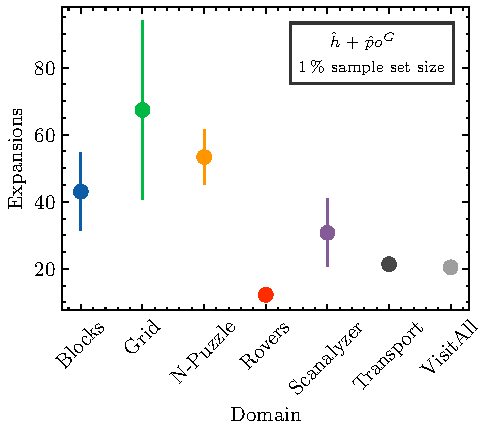
\includegraphics[width=\linewidth]{img/error_hNN_poG_1pct.pdf}
  \end{subfigure}
  %\hfill
  \begin{subfigure}{0.41\textwidth}
    \centering
    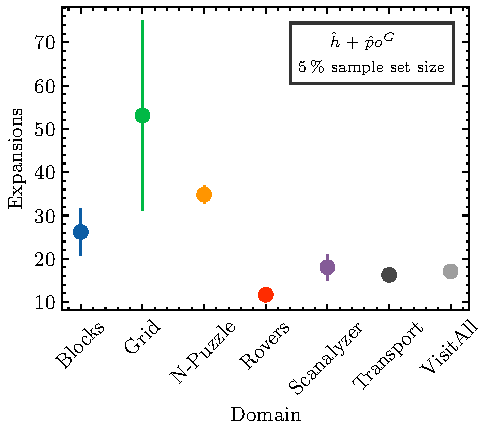
\includegraphics[width=\linewidth]{img/error_hNN_poG_5pct.pdf}
  \end{subfigure}


  \vspace{0.5cm}

  %\hfill
  \begin{subfigure}{0.41\textwidth}
    \centering
    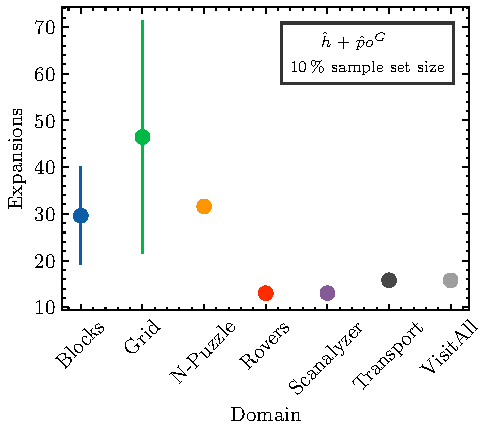
\includegraphics[width=\linewidth]{img/error_hNN_poG_10pct.pdf}
  \end{subfigure}
  \begin{subfigure}{0.41\textwidth}
    \centering
    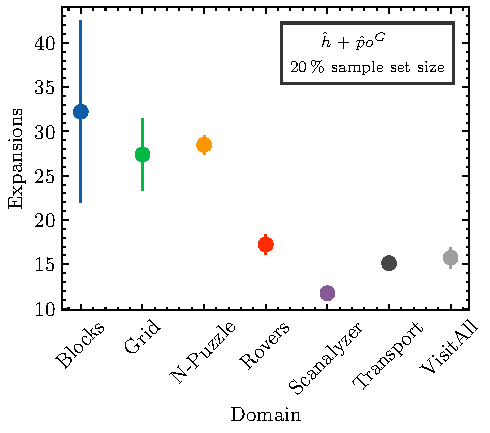
\includegraphics[width=\linewidth]{img/error_hNN_poG_20pct.pdf}
  \end{subfigure}
  %\hfill

  \vspace{0.5cm}

  \begin{subfigure}{0.41\textwidth}
    \centering
    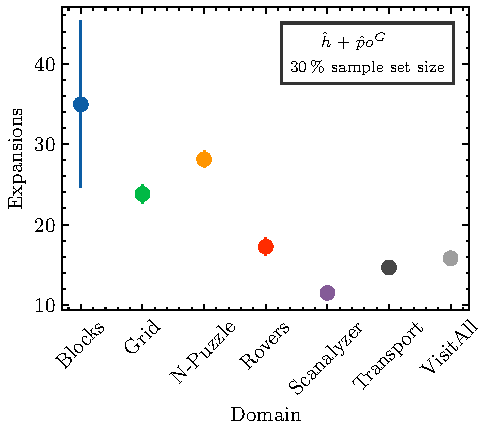
\includegraphics[width=\linewidth]{img/error_hNN_poG_30pct.pdf}
  \end{subfigure}
  %\hfill
  \begin{subfigure}{0.41\textwidth}
    \centering
    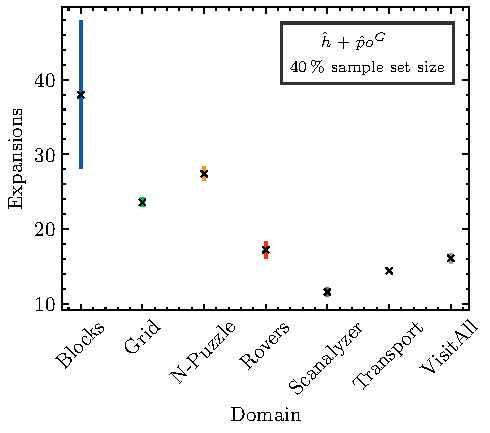
\includegraphics[width=\linewidth]{img/error_hNN_poG_40pct.pdf}
  \end{subfigure}

  \vspace{0.5cm}

  \begin{subfigure}{0.41\textwidth}
    \centering
    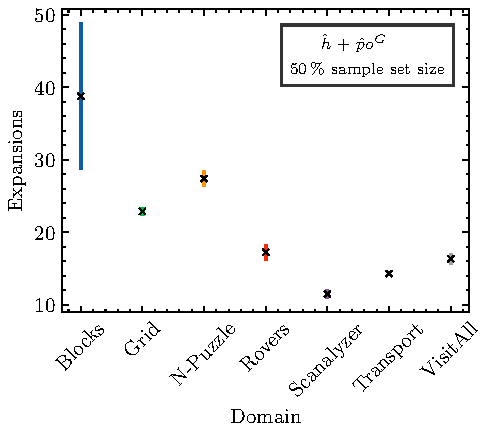
\includegraphics[width=\linewidth]{img/error_hNN_poG_50pct.pdf}
  \end{subfigure}
  \label{fig:errors}
\end{figure}


\section{Comparison to Alternative Sampling Method}
\label{sec:exp-comparison-sample-method}
%\citet{Bettker.etal/2022}~(\cref{sec:sample-learn-h}) propose a sampling generation technique to produce pairs of states and cost-to-goal estimates. Although the method yields satisfactory outcomes for learning heuristic functions, it falls short in acquiring preferred operators.
%This limitation arises from the presence of numerous duplicate sampled states that do not contribute to constructing the shortest path graph $G'$. Consequently, we discover fewer preferred operators than would be possible otherwise.
In this experiment, we compare the number of expansions between two methods for discovering operators. The first method is the sampling approach proposed in \cref{sec:sample-learn-po}, while the second method is the one introduced by~\citet{Bettker.etal/2022} and described in \cref{sec:sample-learn-h} (differently from learning \hnn, we exclude randomly generated samples since they are not necessarily generated by applicable operators).
\cref{tab:comparison_sample} shows the results. The learned preferred operators \pog consistently expands fewer states than \pofsm, except for Blocks World (from $20\,\%$ onwards) and VisitAll. Notably, \pofsm needs ten times the number of samples (e.g., $50\,\%$ vs. $5\,\%$) to achieve comparable results to \pog on average.

\begin{table}[tb]
\centering
%\small
%\setlength{\tabcolsep}{0.9ex}
\caption[Expansions of \pog and \pofsm]{Expansions of GBFS guided by \hnn with \pog and \pofsm using FSM from~\citet{Bettker.etal/2022}, varying the size of the sample set according to different percentages of the forward state space size.}
\label{tab:comparison_sample}
\vspace{\baselineskip}
\begin{tabular}{lrrrrrrrrrr}
\toprule
           &  \multicolumn{2}{c}{$1\,\%$} & \multicolumn{2}{c}{$5\,\%$} & \multicolumn{2}{c}{$10\,\%$} & \multicolumn{2}{c}{$20\,\%$} \\
\cmidrule(lr){2-3} \cmidrule(lr){4-5} \cmidrule(lr){6-7} \cmidrule(lr){8-9}
Domain     &  \pog  & \pofsm & \pog  & \pofsm & \pog & \pofsm & \pog & \pofsm \\ \midrule
Blocks     &  \textbf{43.0}  & 56.8   & \textbf{26.2}  & 31.7 & \textbf{29.6} & 30.4 & \textbf{32.2} & 32.8    \\
Grid       &  \textbf{67.4}  & 74.3   & \textbf{53.0}  & 67.8 & \textbf{46.4} & 67.3 & \textbf{27.4} & 69.9    \\
N-Puzzle   &  \textbf{53.3}  & 67.6   & \textbf{34.8}  & 48.5 & \textbf{31.6} & 38.1 & \textbf{28.5} & 32.3   \\
Rovers     &  12.2  & \textbf{12.1}   & \textbf{11.7}  & 13.1 & \textbf{13.0} & 15.7 & \textbf{17.2} & 19.9   \\
Scanalyzer &  \textbf{30.7}  & 33.7   & \textbf{18.1}  & 21.0 & \textbf{13.0} & 14.5 & \textbf{11.7} & 11.9   \\
Transport  &  \textbf{21.4}  & 23.6   & \textbf{16.3}  & 19.9 & \textbf{15.8} & 18.2 & \textbf{15.1} & 16.9   \\
VisitAll   &  20.5  & \textbf{19.8}   & 17.1  & \textbf{15.6} & 15.7 & \textbf{15.3} & 15.7 & \textbf{14.8}   \\ \midrule
Geo. mean  &  \textbf{30.6}  & 34.2   & \textbf{22.4}  & 26.4 & \textbf{21.0} & 24.3 & \textbf{19.8} & 23.8  \\ \midrule
\end{tabular}

\begin{tabular}{lrrrrrrrrrrrr}
           &  \multicolumn{2}{c}{$30\,\%$} & \multicolumn{2}{c}{$40\,\%$} & \multicolumn{2}{c}{$50\,\%$} &&&&&& \\
\cmidrule(lr){2-3} \cmidrule(lr){4-5} \cmidrule(lr){6-7}
     &   \pog & \pofsm & \pog & \pofsm & \pog & \pofsm &&&&&& \\ \midrule
Blocks     &  34.9 & \textbf{33.2} & 38.0 & \textbf{32.1} & 38.8 & \textbf{32.3} &&&&&& \\
Grid       &  \textbf{23.8} & 64.5 & \textbf{23.6} & 59.1 & \textbf{22.9} & 55.0 &&&&&& \\
N-Puzzle   &  \textbf{28.1} & 29.6 & \textbf{27.4} & 28.9 & \textbf{27.4} & 27.7 &&&&&& \\
Rovers     &  \textbf{17.2} & 20.8 & \textbf{17.2} & 21.3 & \textbf{17.2} & 21.4 &&&&&& \\
Scanalyzer &  \textbf{11.5} & 11.6 & 11.6 & \textbf{11.5} & \textbf{11.5} & 11.7 &&&&&& \\
Transport  &  \textbf{14.7} & 16.1 & \textbf{14.4} & 15.8 & \textbf{14.3} & 15.5 &&&&&& \\
VisitAll   &  15.8 & \textbf{14.9} & 16.1 & \textbf{15.6} & 16.3 & \textbf{15.4} &&&&&& \\ \midrule
Geo. mean  &  \textbf{19.5} & 23.2 & \textbf{19.7} & 22.9 & \textbf{19.6} & 22.5 &&&&&& \\ \bottomrule
\end{tabular}
\end{table}

\iffalse
\begin{table}[!h]
\centering
\small
\setlength{\tabcolsep}{0.9ex}
\caption{Number of expansions GBFS guided by \hnn with \pog and \pofsm, varying the size of the sample set according to different percentages of the state space size.}
\label{tab:comparison_sample}
\vspace{\baselineskip}
\begin{tabular}{lrrrrrrrrrrrrrr}
\toprule
           &  \multicolumn{2}{c}{$1$} & \multicolumn{2}{c}{$5$} & \multicolumn{2}{c}{$10$} & \multicolumn{2}{c}{$20$} & \multicolumn{2}{c}{$30$} & \multicolumn{2}{c}{$40$} & \multicolumn{2}{c}{$50$} \\
\cmidrule(lr){2-3} \cmidrule(lr){4-5} \cmidrule(lr){6-7} \cmidrule(lr){8-9} \cmidrule(lr){10-11} \cmidrule(lr){12-13} \cmidrule(lr){14-15}
Domain     &  \pog  & \pofsm & \pog  & \pofsm & \pog & \pofsm & \pog & \pofsm & \pog & \pofsm & \pog & \pofsm & \pog & \pofsm \\ \midrule
Blocks     &  43.0  & 56.8   & 26.2  & 31.7 & 29.6 & 30.4 & 32.2 & 32.8 & 34.9 & 33.2 & 38.0 & 32.1 & 38.8 & 32.3 \\
Grid       &  67.4  & 74.3   & 53.0  & 67.8 & 46.4 & 67.3 & 27.4 & 69.9 & 23.8 & 64.5 & 23.6 & 59.1 & 22.9 & 55.0 \\
N-Puzzle   &  53.3  & 67.6   & 34.8  & 48.5 & 31.6 & 38.1 & 28.5 & 32.3 & 28.1 & 29.6 & 27.4 & 28.9 & 27.4 & 27.7 \\
Rovers     &  12.2  & 12.1   & 11.7  & 13.1 & 13.0 & 15.7 & 17.2 & 19.9 & 17.2 & 20.8 & 17.2 & 21.3 & 17.2 & 21.4 \\
Scanalyzer &  30.7  & 33.7   & 18.1  & 21.0 & 13.0 & 14.5 & 11.7 & 11.9 & 11.5 & 11.6 & 11.6 & 11.5 & 11.5 & 11.7 \\
Transport  &  21.4  & 23.6   & 16.3  & 19.9 & 15.8 & 18.2 & 15.1 & 16.9 & 14.7 & 16.1 & 14.4 & 15.8 & 14.3 & 15.5 \\
VisitAll   &  20.5  & 19.8   & 17.1  & 15.6 & 15.7 & 15.3 & 15.7 & 14.8 & 15.8 & 14.9 & 16.1 & 15.6 & 16.3 & 15.4 \\ \midrule
Geo. mean  &  30.6  & 34.2   & 22.4  & 26.4 & 21.0 & 24.3 & 19.8 & 23.8 & 19.5 & 23.2 & 19.7 & 22.9 & 19.6 & 22.5 \\ \bottomrule

\end{tabular}
\end{table}
\fi



\section{Using Learned Preferred Operators with Other Heuristic Functions}
\label{sec:other-heuristic-functions}
We now examine the effects of using the learned preferred operators \pog, trained on a $1\,\%$ sample set size, on the performance of GBFS guided by different logic-based heuristic functions. Specifically, we evaluate the effect on the more informed heuristics \hff and \hadd, the less informed heuristic \hgc (goal-count), and Blind search without information. We also compare our results with searches using \poff. The outcomes are summarized in \cref{tab:logic_heuristics_1pct}.

\begin{table}[tb]
\centering
%\setlength{\tabcolsep}{0.8ex}
\caption{Expanded states of GBFS guided by symbolic-based heuristics without preferred operators $h$, and with preferred operators obtained by FF~\poff and the SPG~\pog.}
\label{tab:logic_heuristics_1pct}
\vspace{\baselineskip}
\begin{tabular}{lrrrrrr}
\toprule
        & \multicolumn{3}{c}{$\hff$} & \multicolumn{3}{c}{$\hadd$} \\
\cmidrule(lr){2-4}\cmidrule(lr){5-7}
Domain     & $h$   & \poff & \pog & $h$   & \poff & \pog \\ \midrule
Blocks     & 183.0 & 52.8  & 46.6 & 94.9  & 51.2  & 39.4  \\
Grid       & 33.6  & 30.0  & 30.0 & 48.5  & 33.3  & 30.5  \\
N-Puzzle   & 139.9 & 205.9 & 59.1 & 155.7 & 198.0 & 69.3  \\
Rovers     & 11.5  & 10.6  & 10.6 & 11.4  & 19.0  & 10.6  \\
Scanalyzer & 28.5  & 16.9  & 29.3 & 21.6  & 14.3  & 23.4  \\
Transport  & 17.8  & 15.6  & 19.9 & 17.9  & 16.4  & 20.0  \\
VisitAll   & 27.3  & 23.8  & 20.4 & 30.4  & 29.4  & 19.6  \\ \midrule
Geo. mean  & 39.0  & 30.0  & 27.0 & 37.1  & 33.2  & 26.0  \\ \midrule
\end{tabular}

\begin{tabular}{lrrrrrr}

        &  \multicolumn{3}{c}{$\hgc$} & \multicolumn{3}{c}{Blind} \\
\cmidrule(lr){2-4}\cmidrule(lr){5-7}
     &  $h$   & \poff  & \pog & $h$      & \poff   & \pog \\ \midrule
Blocks     &  332.7 & 62.5   & 60.5 & 54K   & 10K   & 306.8 \\
Grid       &  265.6 & 60.4   & 91.5 & 51K   & 11K   & 152.0 \\
N-Puzzle   &  818.7 & 1.2K   & 77.4 & 67K   & 67K   & 368.3 \\
Rovers     &  61.5  & 17.5   & 21.2 & 4K    & 832.1 & 126.4 \\
Scanalyzer &  31.9  & 18.4   & 28.9 & 5K    & 3K    & 446.1 \\
Transport  &  200.5 & 44.1   & 40.2 & 145K  & 15K   & 193.4 \\
VisitAll   &  16.7  & 13.9   & 19.7 & 2K    & 2K    & 277.5 \\ \midrule
Geo. mean  &  124.9 & 51.3   & 41.4 & 19.7K & 6.7K  & 244.3 \\ \bottomrule
\end{tabular}

\end{table}

\iffalse
\begin{table}[tb]
\centering
\setlength{\tabcolsep}{0.8ex}
\caption{Expanded states of GBFS guided by symbolic-based heuristics without preferred operators $h$, and with preferred operators obtained by FF~\poff and the shortest path graph~\pog.}
\label{tab:logic_heuristics_1pct}
\vspace{\baselineskip}
\begin{tabular}{lrrrrrrrrrrrr}
\toprule
        & \multicolumn{3}{c}{$\hff$} & \multicolumn{3}{c}{$\hadd$} & \multicolumn{3}{c}{$\hgc$} & \multicolumn{3}{c}{Blind} \\
\cmidrule(lr){2-4}\cmidrule(lr){5-7}\cmidrule(lr){8-10}\cmidrule(lr){11-13}
Domain     & $h$   & \poff & \pog & $h$   & \poff & \pog & $h$   & \poff  & \pog & $h$      & \poff   & \pog \\ \midrule
Blocks     & 183.0 & 52.8  & 46.6 & 94.9  & 51.2  & 39.4 & 332.7 & 62.5   & 60.5 & 54K   & 10K   & 306.8 \\
Grid       & 33.6  & 30.0  & 30.0 & 48.5  & 33.3  & 30.5 & 265.6 & 60.4   & 91.5 & 51K   & 11K   & 152.0 \\
N-Puzzle   & 139.9 & 205.9 & 59.1 & 155.7 & 198.0 & 69.3 & 818.7 & 1.2K   & 77.4 & 67K   & 67K   & 368.3 \\
Rovers     & 11.5  & 10.6  & 10.6 & 11.4  & 19.0  & 10.6 & 61.5  & 17.5   & 21.2 & 4K    & 832.1 & 126.4 \\
Scanalyzer & 28.5  & 16.9  & 29.3 & 21.6  & 14.3  & 23.4 & 31.9  & 18.4   & 28.9 & 5K    & 3K    & 446.1 \\
Transport  & 17.8  & 15.6  & 19.9 & 17.9  & 16.4  & 20.0 & 200.5 & 44.1   & 40.2 & 145K  & 15K   & 193.4 \\
VisitAll   & 27.3  & 23.8  & 20.4 & 30.4  & 29.4  & 19.6 & 16.7  & 13.9   & 19.7 & 2K    & 2K    & 277.5 \\ \midrule
Geo. mean  & 39.0  & 30.0  & 27.0 & 37.1  & 33.2  & 26.0 & 124.9 & 51.3   & 41.4 & 19.7K & 6.7K  & 244.3 \\ \bottomrule
\end{tabular}
\end{table}
\fi


Using the learned preferred operators \pog with the \hgc heuristic reduces the number of expansions from $124.9$ to $41.4$. This performance is competitive with the baseline \hff and \hadd heuristics, and it yields fewer expansions in Blocks World, N-Puzzle, and VisitAll. Furthermore, when using \hgc with \pog trained on a $5\,\%$ sample set size, we achieve a geometric mean of $28.1$, which is approximately $25\,\%$ lower than the results obtained with the baseline \hff and \hadd heuristics. These findings highlight that using preferred operators can lead to more significant performance improvements in task-solving compared to changing to a more informed heuristic.


\chapter{Limitations}
\label{cha:limitations}
A clear limitation of learned preferred operators is the number of samples required for training. Our experiments used small state spaces and a relatively simple NN as a first step to explore learning preferred operators. Consequently, we had access to the complete state space of a task. However, this is infeasible for harder tasks, as state spaces tend to grow exponentially in size as the amount of information needed to describe them increases, meaning that if computational resources are a concern, even sampling $1\,\%$ of the state space can be impractical. Another problem involves the size of the output tensor, where certain domains have of thousands of classes in larger tasks, which significantly affects training efficiency.

Therefore, to improve learning efficiency, future research could focus on experimenting with other learning architectures that enable the generalization of preferred operators using a smaller number of samples, or an alternative representation of preferred operators as the target value.

\chapter{Conclusion}
\label{cha:conclusion}
Extensive research has been conducted on learning heuristic functions for solving planning tasks. We explore for the first time the learning of preferred operators. The proposed approaches not only provide novel insights into planning but also have the potential for broader applications beyond planning, such as in reinforcement learning.

The approaches presented in this research are alternatives to policies in reinforcement learning. Despite the lack of an explicit goal state in reinforcement learning, the methods described in this work can be used to learn to seek states that lead to higher rewards over time. By establishing a hierarchy of goals in complex problems, the learning process can be divided into multiple stages with each goal state defined in terms of higher-level objectives. This hierarchical structure enables the agent to sample from multiple goal states and work towards specific goals at different stages.

The findings suggest that learning-based approaches have a considerable potential to outperform logic-based methods. We demonstrate that learned preferred operators can surpass logic-based preferred operators like \poff in the considered planning tasks. Additionally, using less informed heuristics with preferred operators can lead to fewer expanded states compared to switching to more informed heuristics. The experiments highlight the ability to discover preferred operators and train an NN capable of generalizing for the entire task using only a small subset of the complete state space. Analysis between successor and predecessor states proved to be an effective method for discovering preferred operators from a limited sample set.

Overall, this study opens up new possibilities for improving heuristic search in planning through learning of preferred operators and showcases the potential for their application in diverse domains, including reinforcement learning.


\bibliographystyle{abntex2-alf}
\bibliography{biblio}

\appendix


\chapter{Source Code}
Available here. TBA.

\chapter{Tasks of Each Domain}
\label{cha:tasks_each_domain}
The Blocks World domain involves manipulating blocks on a table to achieve a desired configuration through a sequence of actions. We used a planning task with $7$ blocks.

In the Grid domain, an agent traverses a grid, capable of holding a key, with certain cells being locked and requiring specific keys to open. Prior to entering a locked cell. We used a planning task with a $4 \times 4$ grid, four locked cells, and three keys with two possible shapes, circle or square.

The N-Puzzle domain consists of a square grid with numbered tiles. The objective is to rearrange the tiles from their initial scrambled state to a desired goal state. We used a planning task with a $3 \times 3$ grid.

The Rovers domain involves rovers navigating a grid-based environment with missions like exploration or resource gathering. Each rover has specific capabilities and limitations, including movement range, sensing, and interaction abilities. We used a planning task with two rovers, each with one storage capacity and one camera, and four waypoints with different objectives.

The Scanalyzer domain models automated greenhouse logistics, using imaging facilities to collect plant data and conveyor belts to transport plants between smart greenhouses and imaging facilities. We use a planning task with six conveyor belts and six batches of plants.

The Transport domain consists of transporting packages from one location to another using trucks with specific capacities. We use a planning task with nine cities, two trucks, and four packages.

The VisitAll domain consists of a robot that needs to visit all the cells of a grid once. We use a planning task with a $4 \times 4$ grid.


\chapter{Discovered Preferred Operators Without Boosting}
\label{cha:discovered_pos_boost0}
\cref{tab:learning_discovered_pos_boost0} shows the number of expanded states using the discovered preferred operators \pog but no boosting during search, i.e., states are expanded alternately from the default queue and the preferred queue.

\begin{table}[!h]
\centering
\caption[Expansions of \pog without boosting]{Expansions of DQ-GBFS guided by \hnn with \pog trained with the discovered learned operators varying the size of the sample set according to different percentages of the state space size. Boosting is disabled.}
\label{tab:learning_discovered_pos_boost0}
\vspace{\baselineskip}
\begin{tabular}{lrrrrrrr}
\toprule
& \multicolumn{7}{c}{$\pog$} \\
\cmidrule(lr){2-8}
Domain     & $1\,\%$ & $5\,\%$   & $10\,\%$ & $20\,\%$ & $30\,\%$ & $40\,\%$ & $50\,\%$ \\ \midrule
Blocks         & 43.6 & 32.0 & 33.3  & 34.6  & 34.6  & 36.1  & 36.5  \\
Grid           & 63.7 & 55.6 & 47.5  & 35.0  & 31.9  & 31.5  & 30.9  \\
N-Puzzle       & 57.5 & 44.1 & 42.1  & 40.5  & 39.8  & 38.9  & 39.0  \\
Rovers         & 14.0 & 13.4 & 13.5  & 13.3  & 13.3  & 13.3  & 13.3  \\
Scanalyzerunit & 31.1 & 21.6 & 17.2  & 16.1  & 16.0  & 15.8  & 16.3  \\
Transportunit  & 22.4 & 19.7 & 19.3  & 19.1  & 18.7  & 18.6  & 18.4  \\
VisitAll       & 20.0 & 18.9 & 18.2  & 18.2  & 18.0  & 18.1  & 18.6  \\ \midrule
Geo. mean      & 31.6 & 26.2 & 24.6  & 23.2  & 22.7  & 22.7  & 22.9 \\ \bottomrule
\end{tabular}
\end{table}


\chapter{Training Details}
\cref{tab:training_info} presents the mean training information for the learned preferred operators \pog networks across $25$ different seed runs for each domain, trained over sample sets of distinct sizes. The table shows the size of the sample set in relation to the forward state space, the epoch associated with the minimum validation loss, the value of the minimum validation loss, the elapsed time required to train an NN, and the number of preferred operators per sample. All the networks converged.

\begin{table}[!h]
\centering
%\small
%\setlength{\tabcolsep}{0.7ex}
\caption{Training summary over $25$ seeds for each domain, with the goal of learning \pog.} 
\label{tab:training_info}
\vspace{\baselineskip}
\scalebox{0.85}{
\begin{tabular}{lrrrrr}
\toprule
Domain   & Sample set size ($\%$) &  Best epoch &  Val. loss &  Elapsed time (s) &  \# ops./sample \\
\midrule
Blocks   & 1 &       167.9 &      0.0113 &                16.8 &                           1.1 \\
         & 5 &        75.0 &      0.0130 &                53.9 &                           1.2 \\
         & 10 &        52.9 &      0.0118 &                92.9 &                           1.2 \\
         & 20 &        42.2 &      0.0104 &               174.2 &                           1.3 \\
         & 30 &        38.6 &      0.0092 &               252.3 &                           1.3 \\
         & 40 &        39.0 &      0.0083 &               342.7 &                           1.4 \\
         & 50 &        35.4 &      0.0076 &               415.6 &                           1.4 \\ \midrule
Grid     & 1 &       105.5 &      0.0022 &                99.2 &                           1.2 \\
         & 5 &        53.1 &      0.0018 &               378.4 &                           1.3 \\
         & 10 &        45.3 &      0.0016 &               730.3 &                           1.3 \\
         & 20 &        39.2 &      0.0014 &              1448.1 &                           1.3 \\
         & 30 &        35.8 &      0.0013 &              2079.7 &                           1.3 \\
         & 40 &        34.3 &      0.0012 &              2758.8 &                           1.3 \\
         & 50 &        34.5 &      0.0011 &              3449.9 &                           1.3 \\ \midrule
N-Puzzle & 1 &       115.0 &      0.0101 &                39.6 &                           1.0 \\
         & 5 &        57.9 &      0.0069 &               145.5 &                           1.0 \\
         & 10 &        48.6 &      0.0070 &               273.3 &                           1.1 \\
         & 20 &        47.9 &      0.0069 &               557.3 &                           1.1 \\
         & 30 &        44.8 &      0.0069 &               811.0 &                           1.1 \\
         & 40 &        42.8 &      0.0070 &              1093.8 &                           1.1 \\
         & 50 &        39.3 &      0.0070 &              1325.7 &                           1.1 \\ \midrule
Rovers   & 1 &        30.6 &      0.0756 &                62.8 &                           2.1 \\
         & 5 &        24.7 &      0.0735 &               305.7 &                           2.9 \\
         & 10 &        22.8 &      0.0678 &               609.4 &                           3.3 \\
         & 20 &        27.8 &      0.0619 &               966.3 &                           3.4 \\
         & 30 &        27.4 &      0.0618 &               969.2 &                           3.4 \\
         & 50 &        28.2 &      0.0618 &               986.9 &                           3.4 \\ \midrule
Scanalyzer & 1 &       186.9 &      0.0244 &                15.2 &                           1.8 \\
         & 5 &       111.4 &      0.0158 &                54.8 &                           2.5 \\
         & 10 &       107.7 &      0.0133 &               105.6 &                           2.9 \\
         & 20 &       109.7 &      0.0131 &               213.7 &                           3.3 \\
         & 30 &       109.9 &      0.0130 &               323.0 &                           3.6 \\
         & 40 &       110.8 &      0.0132 &               441.9 &                           3.8 \\
         & 50 &       115.0 &      0.0131 &               554.3 &                           4.1 \\ \midrule
Transport & 1 &        80.6 &      0.0041 &               170.6 &                           1.3 \\
         & 5 &        45.7 &      0.0035 &               694.8 &                           1.4 \\
         & 10 &        40.3 &      0.0036 &              1326.4 &                           1.4 \\
         & 20 &        39.6 &      0.0035 &              2728.8 &                           1.4 \\
         & 30 &        39.4 &      0.0036 &              3974.5 &                           1.5 \\
         & 40 &        40.1 &      0.0036 &              5404.9 &                           1.5 \\
         & 50 &        41.0 &      0.0036 &              6433.7 &                           1.5 \\ \midrule
VisitAll & 1 &       196.8 &      0.0258 &                21.8 &                           1.4 \\
         & 5 &       105.7 &      0.0319 &                72.5 &                           1.5 \\
         & 10 &        84.9 &      0.0335 &               130.1 &                           1.5 \\
         & 20 &        75.2 &      0.0339 &               242.3 &                           1.6 \\
         & 30 &        69.5 &      0.0338 &               355.1 &                           1.7 \\
         & 40 &        73.3 &      0.0337 &               431.1 &                           1.7 \\
         & 50 &        74.0 &      0.0333 &               540.4 &                           1.8 \\
\bottomrule
\end{tabular}
}
\end{table}


\chapter{Resumo Expandido}
\noindent
%\textbf{Resolução 02/2021 -- Redação de Teses e Dissertações em Inglês}
%Dissertações de Mestrado e Teses de Doutorado do PPGC, bem como outros
%trabalhos escritos tais como Proposta de Tese e PEP, poderão ser
%redigidas em inglês desde que contenham um título e resumo expandido
%redigidos em português. O resumo expandido deve conter no mínimo duas
%páginas inteiras, deve aparecer como apêndice e deve conter as
%principais contribuições e resultados do trabalho.

No contexto de tarefas de planejamento, os agentes precisam a selecionar a melhor ação possível dentre um conjunto consideravelmente vasto de opções disponíveis em cada etapa. Planejadores lógicos têm sido usados para lidar com esse problema, aplicando operadores preferidos que reduzem significativamente a quantidade de ações a serem consideradas. Os planejadores lógicos que incorporam operadores preferidos na busca foram os vencedores da trilha \emph{satisficing} da \emph{International Planning Competition} (IPC) em 2004, 2008, 2011 e 2018~\cite{Helmert/2006,Richter.lama.etal/2011,Richter.lama.etal/2011,Seipp-fast.etal/2018}.
No entanto, este trabalho apresenta um método que vai além dessas abordagens convencionais, introduzindo uma estratégia de amostragem e aprendizado de operadores preferidos com aplicabilidade em todo o espaço de estados de uma tarefa de planejamento.

O objetivo principal deste trabalho é identificar os operadores preferidos ideais, que se encontram nos caminhos mais curtos que levam a um objetivo específico. O desafio reside no fato de que os espaços de estado geralmente são extremamente grandes, o que dificulta a exploração completa de todas as possibilidades. Para contornar essa limitação, desenvolvemos uma nova abordagem de amostragem adaptada, projetada para extrair operadores preferidos de alta qualidade de um conjunto de amostras que representa apenas uma fração do espaço de estados completo. Os resultados demonstraram que essa abordagem reduzida ainda é capaz de alcançar excelentes desempenhos em tarefas de planejamento.

%Uma contribuição importante deste estudo é a aplicação de redes neurais para aproximar efetivamente os operadores preferidos ideais. Por meio do treinamento dessas redes em amostras selecionadas, foi possível obter estimativas precisas dos operadores preferidos para tarefas envolvendo múltiplos estados. Destacamos tambem o potencial de aplicação desta abordagem em outros domínios, como aprendizagem de máquina, como uma alternativa a aprender políticas.

Para fornecer uma análise mais abrangente dessa nova categoria de operadores preferidos, realizamos experimentos controlados. Comparamos sistematicamente os resultados com abordagens lógicas tradicionais como os operadores preferidos do Fast-Forward (FF)~\cite{Hoffmann.Nebel/2001, Helmert/2006}, avaliamos a eficácia dos operadores preferidos aprendidos em diferentes tamanhos de amostra e exploraramos seu desempenho ao serem combinados com diversas funções heurísticas, tanto aprendidas quanto lógicas. Essa investigação detalhada permite uma compreensão mais profunda das vantagens e limitações dos operadores preferidos aprendidos.

Este estudo representa a primeira tentativa de descobrir operadores preferidos a partir de um conjunto de amostras e usar uma NN para aprendê-los. Apresentamos um novo método de amostragem e uma nova técnica para identificar operadores preferidos em amostras. A técnica de amostragem envolve regressão do estado objetivo, construindo um gráfico com estados amostrados que representam suas relações sucessor-predecessor e determinando, para cada estado, o conjunto de operadores usados para atingir o estado objetivo no menor caminho como operadores preferidos. Este estudo revela que uma rede neural pode aprender os operadores preferidos a partir de um subconjunto do espaço de estados e estender esse aprendizado de forma eficaz a todo o espaço de estados em diversos domínios de planejamento. A abordagem proposta supera o melhor método atual de operadores preferidos do FF nas tarefas de referência. Em particular, este trabalho apresenta:

\begin{itemize}
\item Um novo método de amostragem adaptado para descobrir operadores preferidos.
\item Um novo método baseado em gráficos de caminho mais curto para descobrir operadores preferidos em um conjunto de amostras existente.
\item Uma análise da qualidade dos operadores preferidos aprendidos e uma comparação com os métodos baseados em símbolos existentes.
\end{itemize}

Um exemplo de resultado consiste em uma rede treinada sobre uma quantidade de amostras equivalente a $5\,\%$ do espaço de estados completo de uma tarefa. Nesse caso, os operadores preferidos aprendidos superam significativamente uma busca guiada apenas por uma heurística aprendida, com diminuição de $36\,\%$ em número de estados expandidos. Além disso, eles também superam os operadores do FF em média, com aproximadamente $20\,\%$ de expansões a menos.

\end{document}
